\clearpage
\section{التطبيقات والتنقل}
\label{sec:builder-feature-navigation}

تحدد صفحة «التطبيقات والتنقل» ما يراه الأعضاء في قائمة التطبيقات وترتيبه. وتعرض التنقل شجرةً من ثلاثة مستويات: التطبيق، ثم أقسامه، ثم الوحدات داخل كل قسم. والوحدة هي أي عنصر يفتحه العضو من القائمة: نوع سجلات أو نموذج أو لوحة معلومات أو صفحة أو صفحة مضمّنة في النظام.

ومن هذه الصفحة تعيد ترتيب العناصر بالسحب، وتُظهرها أو تخفيها بمفاتيح التشغيل. ولا تصل هذه التعديلات إلى الأعضاء فوراً، بل تبقى مسودة في الصفحة حتى تضغط «حفظ التغييرات»، فتستطيع أن تجرّب الترتيب وتتراجع عنه بأمان.

\textbf{المسار ومن يستخدمه:} «ادوات البناء» ← «الأساسية» ← «التطبيقات والتنقل». تظهر لمالك المؤسسة ومسؤولها فقط.

\begin{rcnote}[مثال: شركة الأفق]
يضيف مسؤول النظام تطبيق «خدمات الفروع» وقسماً فيه باسم «الزيارات»، ثم يسحب «طلبات الزيارة» إليه ويحفظ، فيجده عمر حداد في قائمة التطبيقات عند فتح الصفحة التالية. ويضيف التطبيق من ① ويحفظ من ⑤.
\end{rcnote}

\begin{figure}[H]
\centering
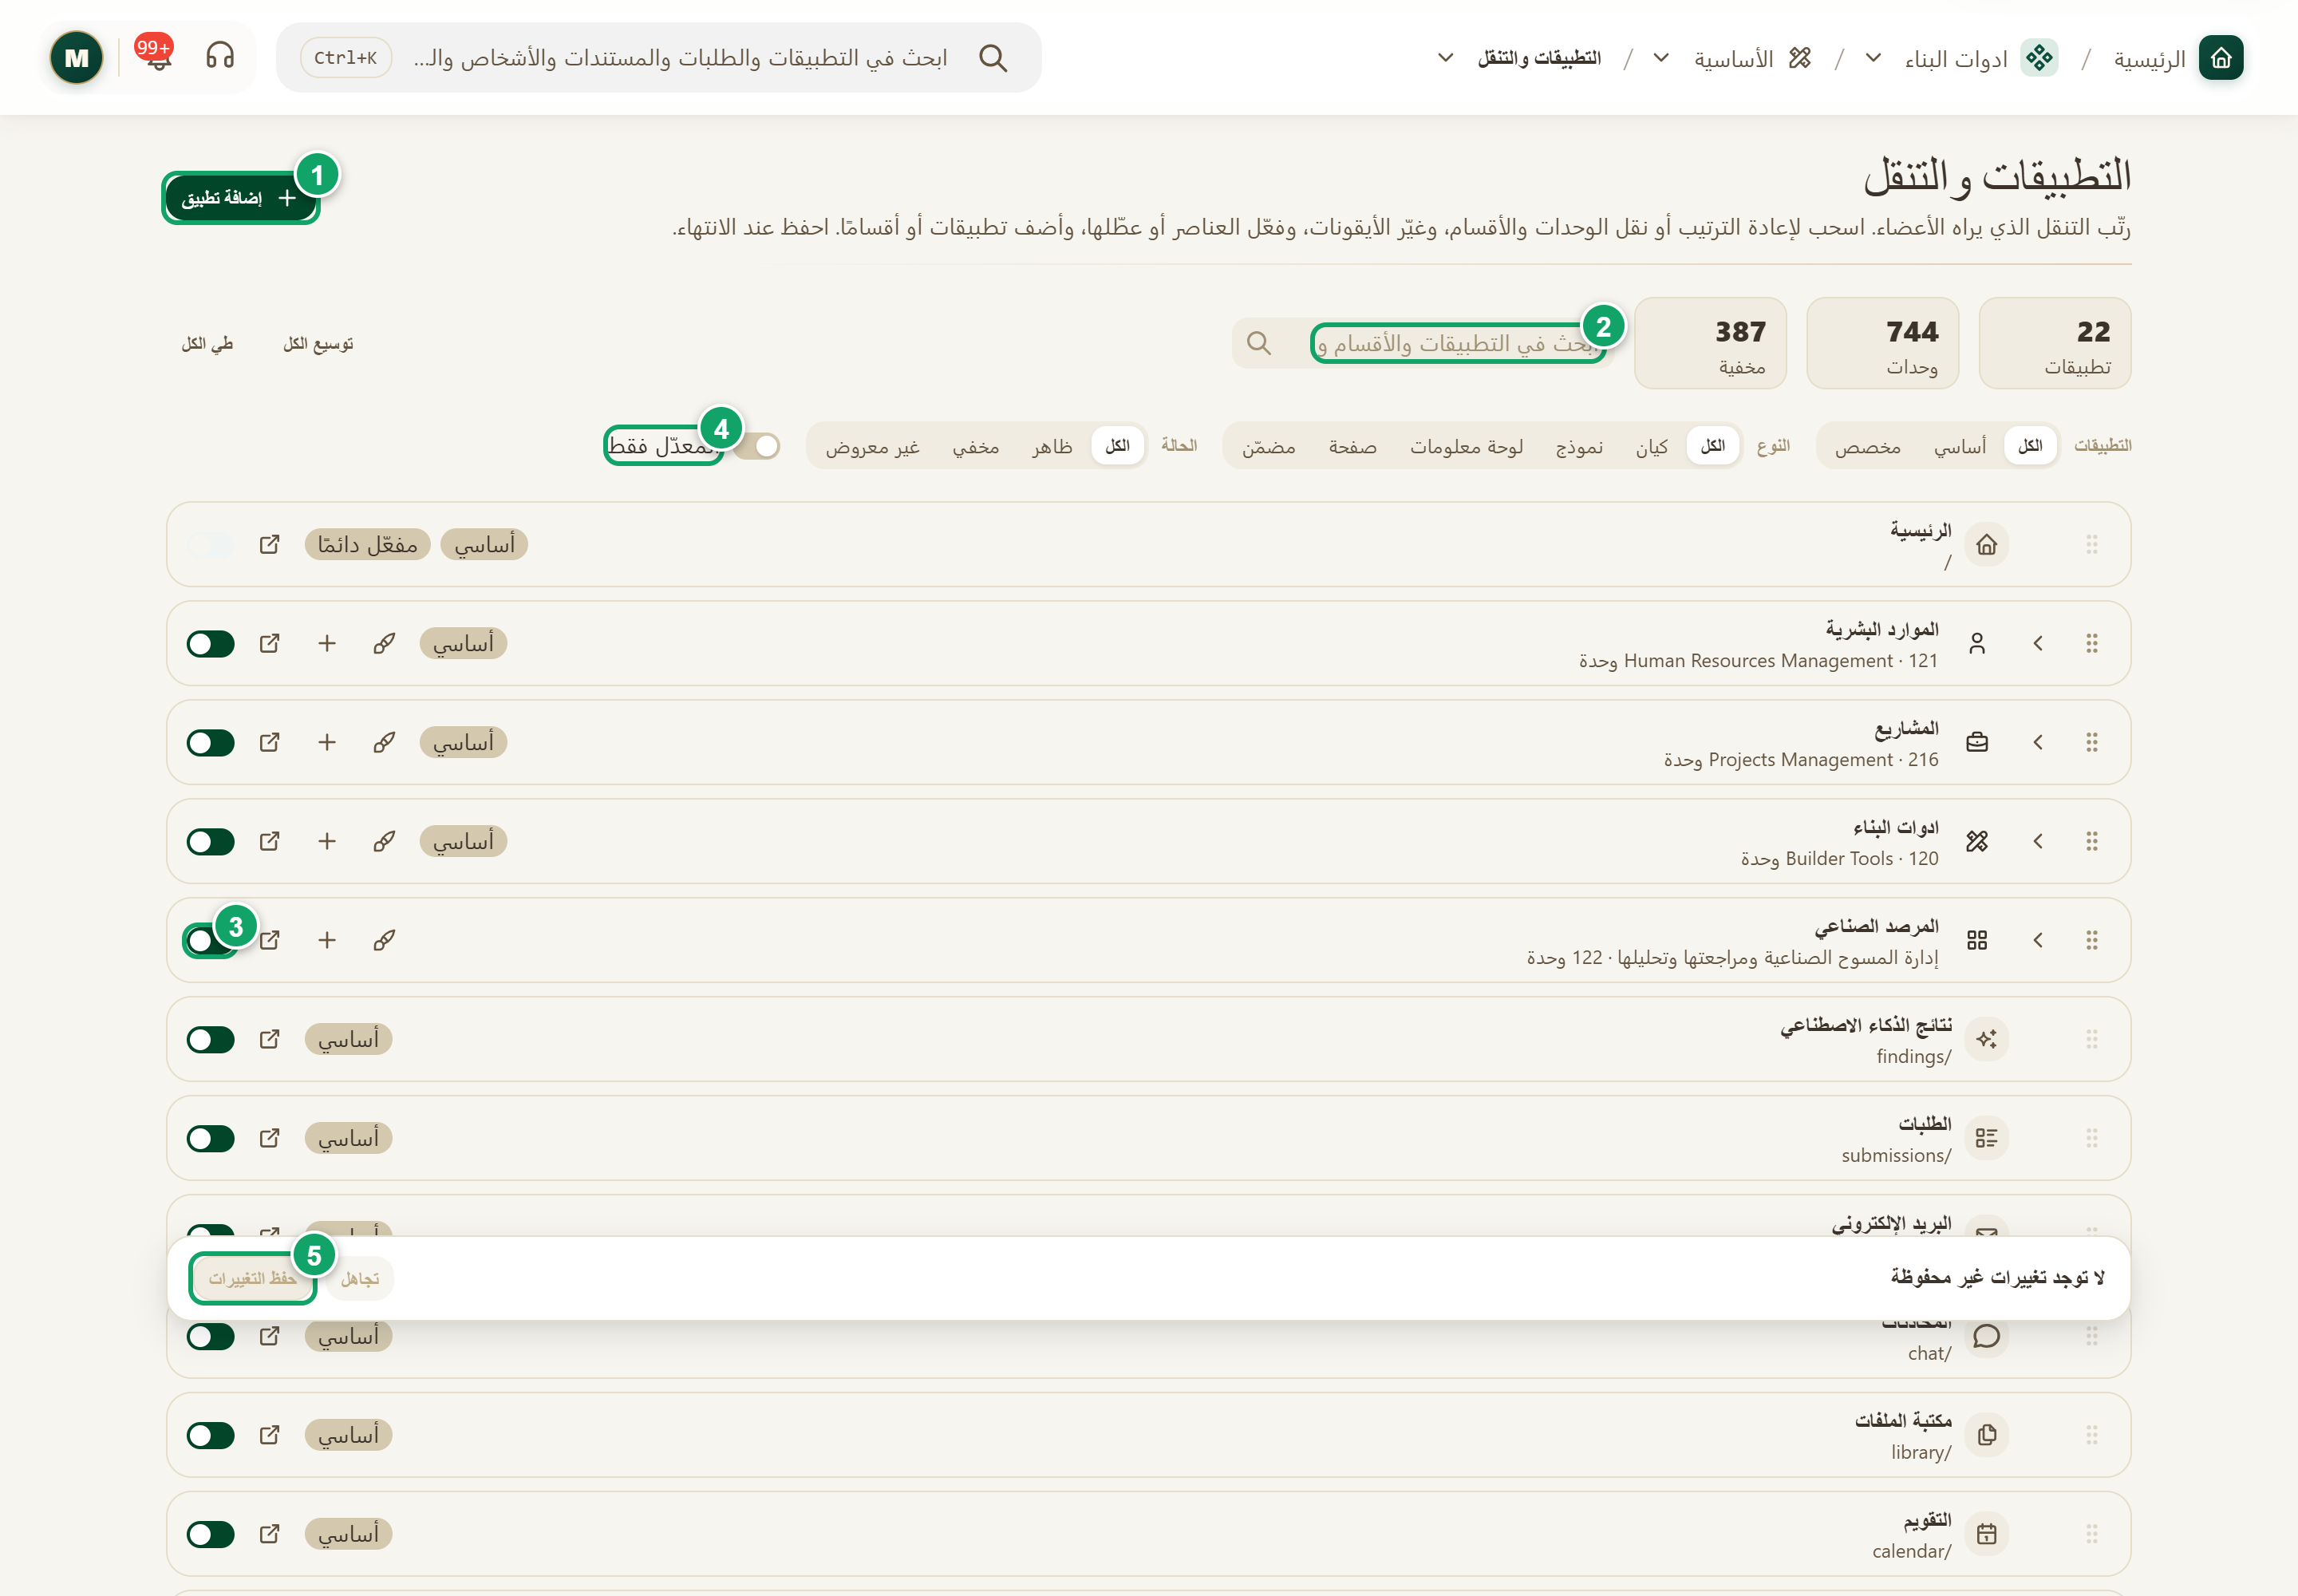
\includegraphics[width=0.95\linewidth,height=0.72\textheight,keepaspectratio]{figures/screens/ch06-navigation-ar.png}
\caption{صفحة «التطبيقات والتنقل»}
\label{fig:builder-navigation-screen}
\shotnote{تعرض الصورة صفحة «التطبيقات والتنقل» في مؤسسة الاختبار، وفيها 22 تطبيقاً لكل منها شاراته ومفتاح ظهوره. وتبقى تغييرات الترتيب والتفعيل مسودة يعرض شريط الحفظ حالتها حتى تحفظها، فتستطيع مراجعتها قبل أن تصل إلى الأعضاء. ① «إضافة تطبيق»: يُنشئ تطبيقاً جديداً ويحفظه فوراً. ② البحث: يجد التطبيق أو القسم أو الوحدة باسمه. ③ مفتاح التطبيق: يُظهره أو يخفيه مع كل ما فيه. ④ «المعدّل فقط»: يعرض ما غيّرته ولم تحفظه. ⑤ «حفظ التغييرات»: يحفظ الترتيب والتفعيل.}
\end{figure}

\begin{table}[H]
\centering
\caption{أجزاء الصفحة}
\label{tab:builder-navigation-data}
\begin{tabularx}{\linewidth}{R{3.6cm} Y}
\rcHeaderRow
\thh{الجزء} & \thh{المحتوى والإجراء}\\
الأرقام والبحث & تعرض الصفحة عدد «تطبيقات» و«وحدات» والعناصر «مخفية». ويجد البحث «ابحث في التطبيقات والأقسام والوحدات» أي عنصر باسمه، ويفتح «توسيع الكل» و«طي الكل» التطبيقات أو يطويها.\\
التصفية & «التطبيقات»: «الكل» أو «أساسي» أو «مخصص»؛ و«النوع»: «كيان» أو «نموذج» أو «لوحة معلومات» أو «صفحة» أو «مضمّن»؛ و«الحالة»: «ظاهر» أو «مخفي» أو «غير معروض»؛ ثم «المعدّل فقط» لعرض ما غيّرته ولم تحفظه. ويعيد «مسح عوامل التصفية» القائمة كاملة.\\
السحب & اسحب التطبيق من مقبضه لتغيّر ترتيبه، واسحب القسم داخل تطبيقه أو إلى تطبيق آخر، واسحب الوحدة داخل قسمها أو إلى قسم آخر.\\
مفاتيح التشغيل & يُظهر المفتاح العنصر أو يخفيه. وإخفاء التطبيق أو القسم يخفي كل ما فيه.\\
شريط الحفظ & يعرض عدد التغييرات غير المحفوظة، وفيه «تجاهل» للتراجع عنها و«حفظ التغييرات» لحفظها.\\
كيف تسري التغييرات & يذكّرك بأن الوحدات تحفظ ظهورها في سجلاتها: أنواع السجلات والنماذج ولوحات المعلومات في «إظهار في التنقل»، والصفحات في حالة نشرها.\\
\end{tabularx}
\end{table}

\begin{table}[H]
\centering
\caption{الشارات في صفوف الشجرة}
\label{tab:builder-navigation-chips}
\begin{tabularx}{\linewidth}{R{3.6cm} Y}
\rcHeaderRow
\thh{الشارة} & \thh{معناها}\\
أساسي & تطبيق مضمّن في النظام، مثل البريد والدردشة. وهذه التطبيقات تُفعَّل أو تُعطَّل فقط، ولا تستقبل وحدات جديدة.\\
مفعّل دائمًا & تطبيق لا يمكن إيقافه، مثل الإعدادات والصفحة الرئيسية، لذلك يكون مفتاحه معطلاً.\\
مخفي أو مسودة & الوحدة نفسها متوقفة. وتظهر «مسودة» للصفحة التي لم تُنشر بعد.\\
معطّل · موروث & الوحدة مفعّلة، لكن تطبيقها أو قسمها متوقف، فلا يراها الأعضاء حتى تشغّل العنصر الأعلى.\\
\end{tabularx}
\end{table}

\begin{rcwarn}[إلى أين يمكن نقل الوحدة؟]
لا يمكن نقل الوحدة إلا إلى قسم له سجل، أي قسم أُضيف من هذه الصفحة أو حُفظ كسجل. فإذا أفلتّ وحدة في قسم مضمّن، تظهر رسالة «هذا التطبيق أو القسم مضمّن ولا يمكنه استقبال وحدات. انقلها إلى قسم له سجل.»، ولا يتغير شيء. أما الوحدات المضمّنة التي لا سجل لها فلا تُسحب أصلاً، ويمكنك إخفاؤها فقط.
\end{rcwarn}

\begin{figure}[H]
\centering
\begin{tikzpicture}[node distance=0.5cm]
\node[entity] (app) {\RL{التطبيق}};
\node[entity,below=0.7cm of app] (section) {\RL{القسم}};
\node[entityOpt,below right=0.7cm and 0.3cm of section] (type) {\RL{نوع سجلات أو نموذج}};
\node[entityOpt,below left=0.7cm and 0.3cm of section] (dash) {\RL{لوحة معلومات أو صفحة}};
\draw[dependsOn] (app) -- (section);
\draw[dependsOnOpt] (section.south) -- ++(0,-0.3) -| (type.north);
\draw[dependsOnOpt] (section.south) -- ++(0,-0.3) -| (dash.north);
\end{tikzpicture}
\rclegend
\caption{كيف يُبنى التنقل}
\label{fig:builder-navigation-tree}
\shotnote{يوضّح الشكل أن التطبيق يضم أقساماً، وأن القسم يضم الوحدات التي يفتحها الأعضاء، مثل أنواع السجلات والنماذج ولوحات المعلومات. لذلك أنشئ التطبيق والقسم أولاً ثم اسحب الوحدة إليه؛ فالتطبيق المضمّن لا يستقبل وحدات جديدة.}
\end{figure}

\subsection{خطوات العمل والتحقق}
\begin{enumerate}
\item افتح «التطبيقات والتنقل»، واكتب اسم الوحدة في البحث، أو اختر نوعها من تصفية «النوع».
\item اسحب الوحدة من مقبضها إلى القسم المطلوب، وأفلتها في الموضع الذي تريده بين وحداته.
\item تأكد من أن مفتاح الوحدة ومفتاحَي قسمها وتطبيقها مشغّلة، وأن الصف لا يحمل شارة «مخفي» أو «معطّل · موروث».
\item فعّل «المعدّل فقط» لتراجع ما غيّرته، ثم اضغط «حفظ التغييرات».
\end{enumerate}

\textbf{تحقق ومعالجة المشكلة:} يجب أن تظهر رسالة «تم حفظ التنقل.»، وأن يعود الشريط إلى «لا توجد تغييرات غير محفوظة»، ثم يرى الأعضاء الترتيب الجديد عند تحميل الصفحة التالي. فإذا لم يظهر العنصر لعضو، فتأكد من أن لديه صلاحية رؤية سجلاته، لأن القسم الذي لا يحتوي عنصراً مسموحاً له لا يظهر. وإذا ظهرت رسالة «تعذّر حفظ التغييرات. يرجى المحاولة مرة أخرى.»، فتحقق من اتصالك واضغط «حفظ التغييرات» مرة أخرى؛ فتعديلاتك تبقى في الصفحة ما لم تضغط «تجاهل».

\clearpage
\section{إضافة التطبيقات والأقسام}
\label{sec:builder-feature-navigation-apps-sections}

عندما تبني عملاً جديداً، فقد لا يناسبه أي تطبيق موجود. لذلك تتيح لك الصفحة إنشاء تطبيق جديد يجمع هذا العمل، ثم إضافة أقسام داخله تصنّف وحداته. ويختلف هذا الإجراء عن الترتيب والتفعيل في أنه يُحفظ فوراً عند الإنشاء، فلا تحتاج بعده إلى «حفظ التغييرات».

ويكفي لكل تطبيق أو قسم عنوانٌ ووصفٌ قصير وأيقونة. ويمكنك لاحقاً تغيير الأيقونة من صفه، وحذف القسم الذي أضفته إذا بقي فارغاً.

\textbf{المسار ومن يستخدمه:} «ادوات البناء» ← «الأساسية» ← «التطبيقات والتنقل» ← «إضافة تطبيق»، أو زر «إضافة قسم» في صف التطبيق. يستخدمه مالك المؤسسة ومسؤولها عند إطلاق عمل جديد.

\begin{rcnote}[مثال: شركة الأفق]
يضغط مسؤول النظام «إضافة تطبيق» ويكتب العنوان «خدمات الفروع» مع وصف يقول إنه يجمع خدمات فرعَي دمشق وحلب، ثم يضغط «إنشاء». بعد ذلك يضيف في التطبيق قسماً باسم «الزيارات» ليضع فيه «طلبات الزيارة». وتطابق هذه الخطوات الأرقام من ① إلى ④ في الصورة.
\end{rcnote}

\begin{figure}[H]
\centering
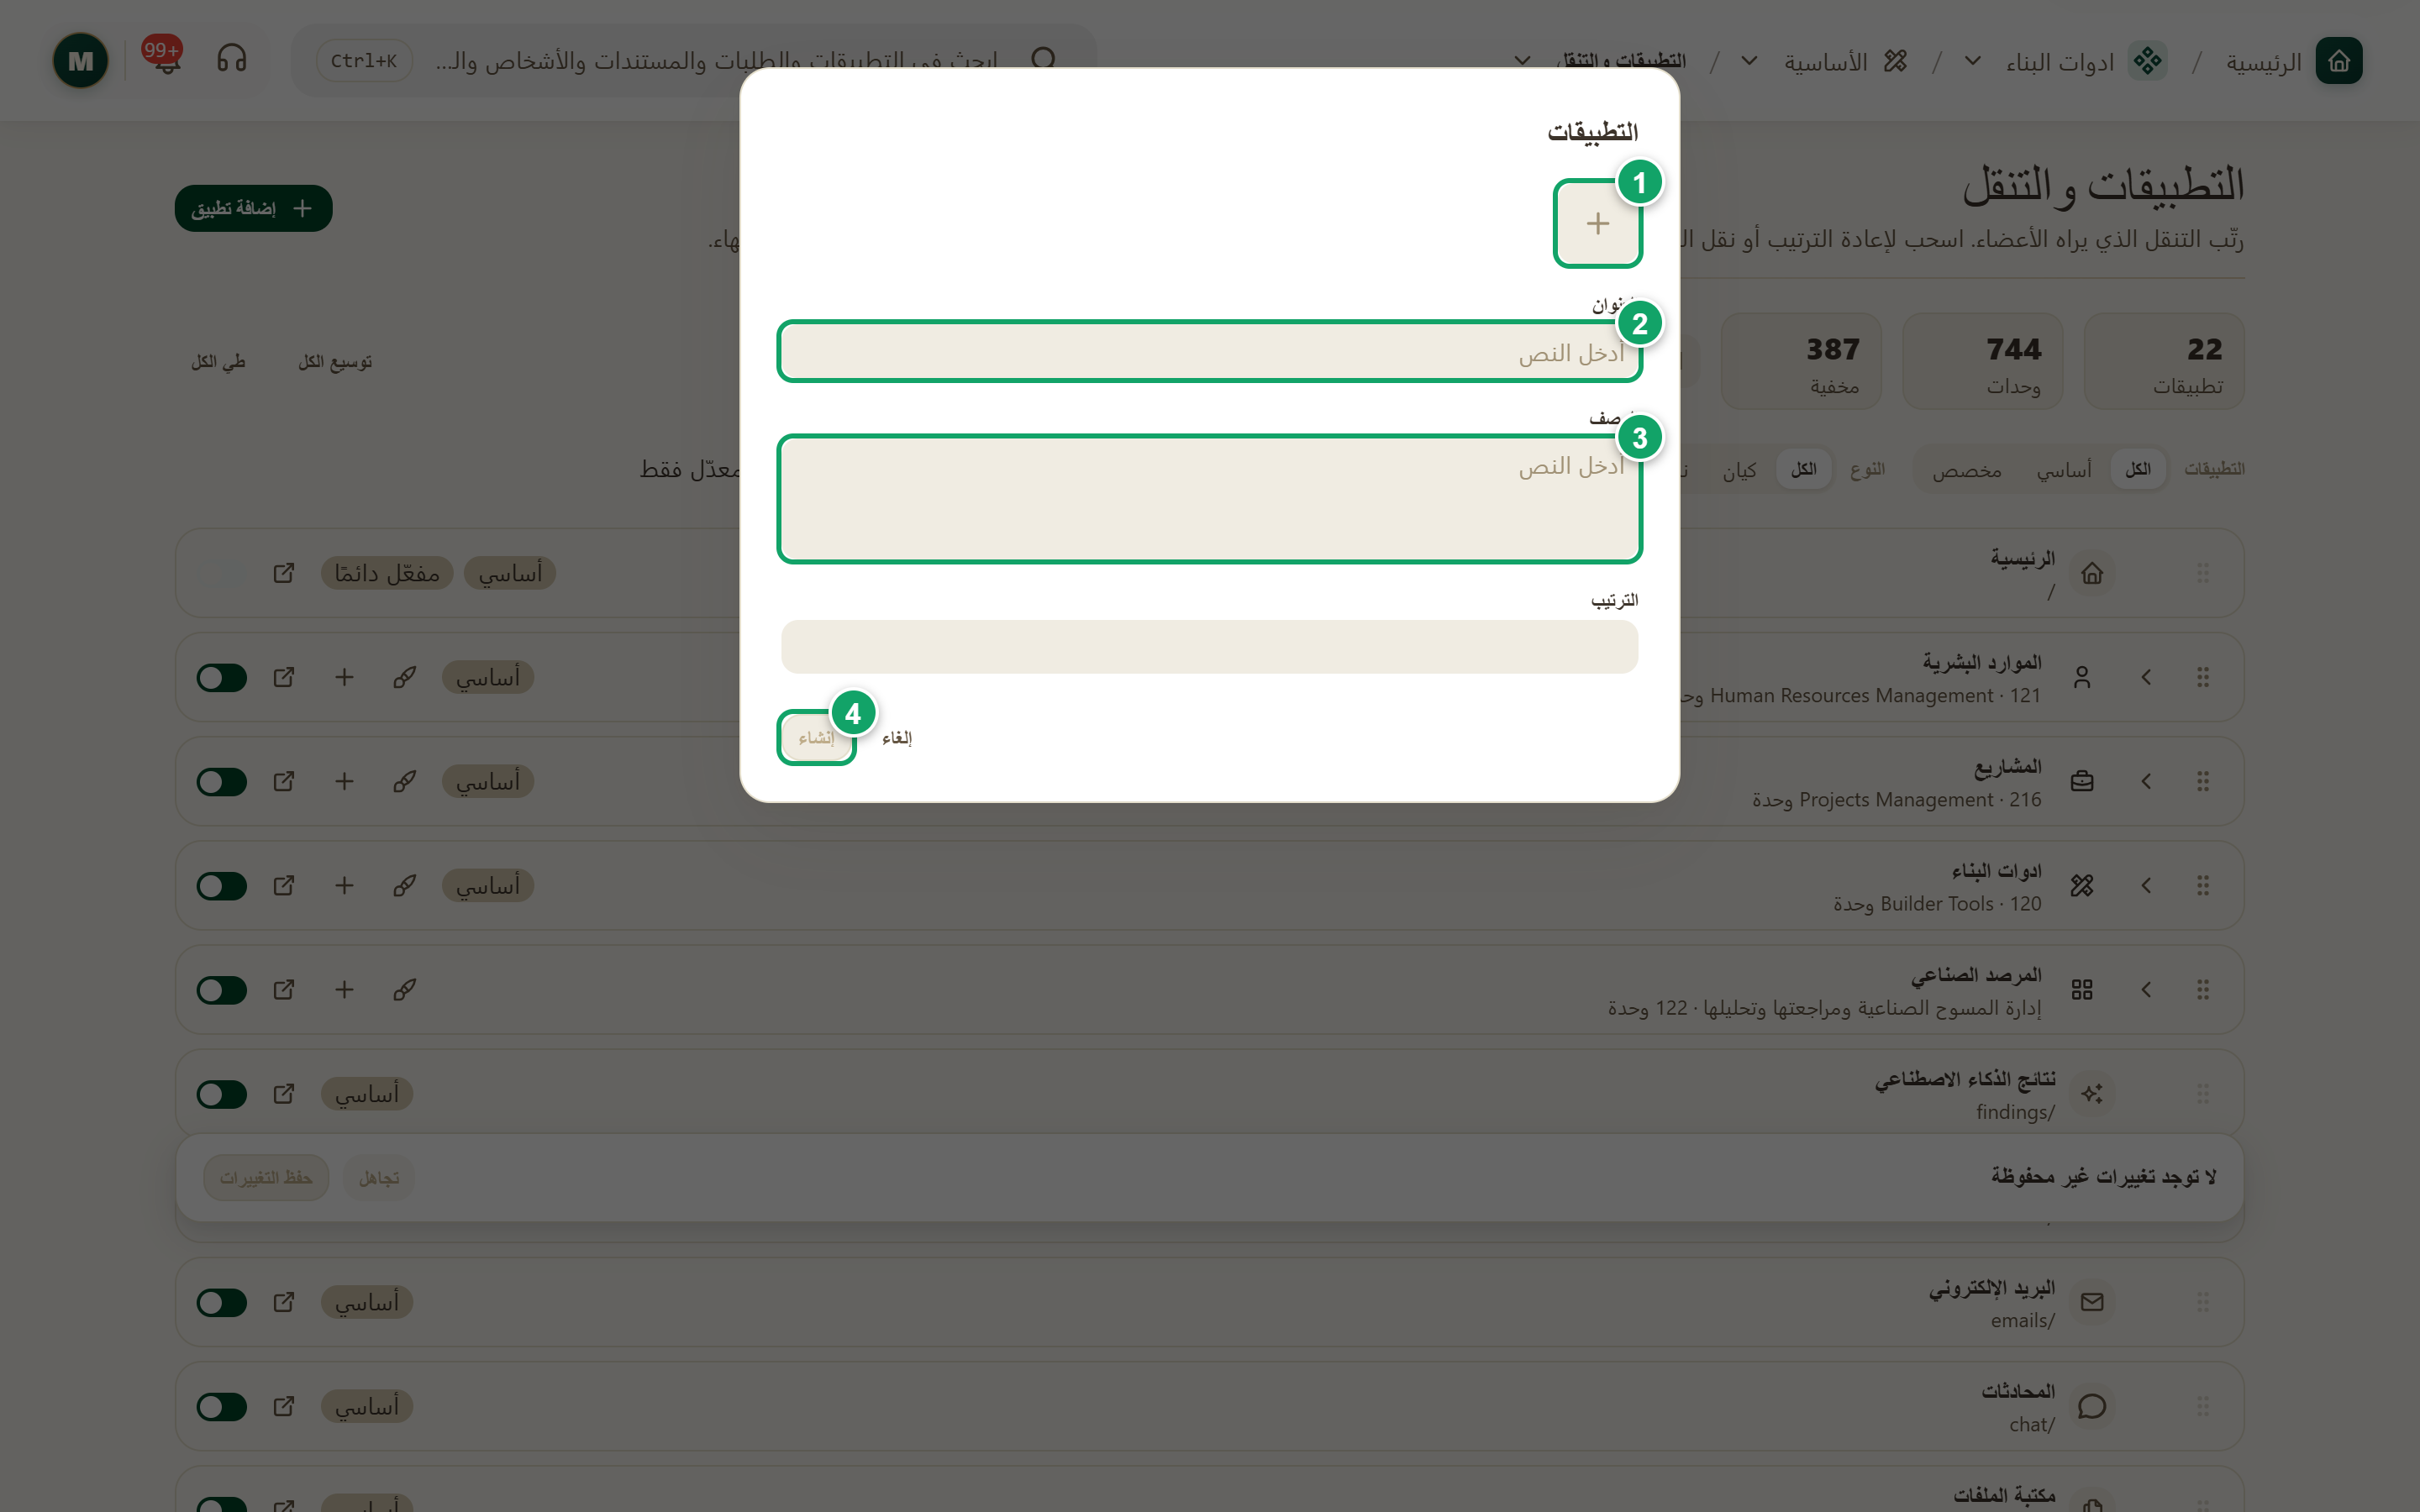
\includegraphics[width=0.95\linewidth,height=0.72\textheight,keepaspectratio]{figures/screens/ch06-nav-add-app-ar.png}
\caption{نافذة إنشاء تطبيق قبل تعبئتها}
\label{fig:builder-navigation-apps-sections-screen}
\shotnote{تعرض الصورة النافذة التي تفتح بعد الضغط على «إضافة تطبيق» في مؤسسة الاختبار، وهي فارغة لأن الالتقاط لم يُنشئ شيئاً. وتفتح النافذة نفسها من زر «إضافة قسم» في صف التطبيق، ويُحفظ ما تنشئه فور الضغط على «إنشاء» دون «حفظ التغييرات». ① منتقي الأيقونة: يختار أيقونة التطبيق أو القسم. ② «العنوان»: الاسم الذي يظهر في القائمة. ③ «الوصف»: جملة إلزامية من 12 حرفاً وكلمتين على الأقل. ④ «إنشاء»: يبقى معطلاً حتى يكتمل العنوان والوصف.}
\end{figure}

\begin{table}[H]
\centering
\caption{نافذة الإنشاء}
\label{tab:builder-navigation-apps-sections-dialog}
\begin{tabularx}{\linewidth}{R{3.6cm} Y}
\rcHeaderRow
\thh{الحقل} & \thh{ما تكتبه فيه}\\
الأيقونة & اختر أيقونة من المنتقي. وإذا لم تختر شيئاً، يأخذ التطبيق أو القسم أيقونة افتراضية.\\
العنوان & الاسم الذي يظهر في القائمة، ويمكن كتابته بكل لغة. وهو حقل إلزامي.\\
الوصف & جملة تشرح الغرض، وهي إلزامية أيضاً. ويجب أن تتكون من 12 حرفاً وكلمتين على الأقل، وإلا ظهرت «صِف في 12 حرفاً وكلمتين على الأقل.».\\
الترتيب & رقم اختياري يحدد موضع العنصر بين نظرائه. ويمكنك تعديل الموضع لاحقاً بالسحب.\\
إنشاء وإلغاء & يبقى «إنشاء» معطلاً حتى تكتب العنوان ووصفاً صالحاً، أما «إلغاء» فيغلق النافذة دون حفظ.\\
\end{tabularx}
\end{table}

\begin{table}[H]
\centering
\caption{أزرار الصف بعد الإنشاء}
\label{tab:builder-navigation-apps-sections-row}
\begin{tabularx}{\linewidth}{R{3.6cm} Y}
\rcHeaderRow
\thh{الزر} & \thh{ما يفعله}\\
إضافة قسم & يظهر في صف التطبيق الذي له سجل، ويفتح النافذة نفسها لإنشاء قسم داخله. ولا يظهر في التطبيقات المضمّنة التي لا أقسام لها.\\
تغيير الأيقونة & يظهر عند أيقونة التطبيق أو القسم أو الوحدة. والأيقونة الجديدة تدخل المسودة، فتحتاج إلى «حفظ التغييرات».\\
حذف القسم & يظهر فقط للقسم الذي أُضيف من هذه الصفحة ولا يحتوي أي وحدة. ويُحذف فوراً للجميع بعد التأكيد، ولا يمكن التراجع عن ذلك.\\
\end{tabularx}
\end{table}

\begin{figure}[H]
\centering
\begin{tikzpicture}[node distance=0.5cm]
\node[stepBox] (a) {\RL{إضافة تطبيق}};
\node[stepBox,below=of a] (b) {\RL{العنوان والوصف والأيقونة}};
\node[stepBox,below=of b] (c) {\RL{إنشاء}};
\node[stepBox,below=of c] (d) {\RL{إضافة قسم في صف التطبيق}};
\node[stepBox,below=of d] (e) {\RL{سحب الوحدات إلى القسم}};
\node[stepBox,below=of e] (f) {\RL{حفظ التغييرات}};
\draw[flowsTo] (a) -- (b);
\draw[flowsTo] (b) -- (c);
\draw[flowsTo] (c) -- (d);
\draw[flowsTo] (d) -- (e);
\draw[flowsTo] (e) -- (f);
\end{tikzpicture}
\rclegend
\caption{من تطبيق جديد إلى قائمة جاهزة}
\label{fig:builder-navigation-apps-sections-flow}
\shotnote{يجمع المخطط نوعين من الحفظ: فالتطبيق والقسم يُحفظان عند الضغط على «إنشاء»، أما نقل الوحدات إلى القسم فيبقى مسودة حتى «حفظ التغييرات». لذلك لا تكتمل القائمة الجديدة إلا بعد الخطوة الأخيرة، لأن القسم الفارغ لا يعرض للأعضاء شيئاً.}
\end{figure}

\subsection{خطوات العمل والتحقق}
\begin{enumerate}
\item افتح «التطبيقات والتنقل» واضغط «إضافة تطبيق».
\item اختر أيقونة، واكتب «العنوان» و«الوصف»، ثم اضغط «إنشاء».
\item ابحث عن التطبيق الجديد، واضغط زر «إضافة قسم» في صفه، واملأ النافذة بالطريقة نفسها، ثم اضغط «إنشاء».
\item اسحب الوحدات إلى القسم الجديد، واضغط «حفظ التغييرات».
\item إذا أنشأت قسماً بالخطأ وبقي فارغاً، فاضغط زر حذفه في صفه، ثم «حذف» في نافذة التأكيد.
\end{enumerate}

\textbf{تحقق ومعالجة المشكلة:} بعد إنشاء القسم تظهر رسالة «تمت إضافة القسم وحفظه مباشرةً، فلا حاجة للضغط على حفظ.»، ويظهر القسم تحت تطبيقه مع العبارة «لا توجد وحدات في هذا القسم. اسحب وحدة إلى هنا.». فإذا بقي «إنشاء» معطلاً، فأطل الوصف ليصبح جملة واضحة. وإذا لم تجد زر الحذف في قسم ما، فإما أن القسم مضمّن أو أن فيه وحدات؛ فانقل وحداته أولاً واحفظ، ثم احذفه.

\clearpage
\section{هوية التطبيق}
\label{sec:builder-feature-navigation-identity}

تمنح «هوية التطبيق» التطبيقَ اسماً وشعاراً ولوناً خاصاً به. فعندما يعمل العضو داخل هذا التطبيق، تحل هويته محل هوية المؤسسة في الشريط العلوي، ثم تعود هوية المؤسسة في بقية الأماكن. ويفيد ذلك عندما يخدم التطبيق جهة أو عميلاً بعينه، فيعرف المستخدم أين يعمل.

وتضم النافذة أيضاً «الوضع المركّز»، وهو يقصر ما يراه بعض الأعضاء على هذا التطبيق وحده. وتُحفظ الهوية فور الضغط على «حفظ» في النافذة، دون الحاجة إلى «حفظ التغييرات».

\textbf{المسار ومن يستخدمه:} «ادوات البناء» ← «الأساسية» ← «التطبيقات والتنقل» ← زر «هوية التطبيق» في صف التطبيق. يظهر الزر للتطبيقات التي لها سجل، ويستخدمه مالك المؤسسة ومسؤولها.

\begin{rcnote}[مثال: شركة الأفق]
يفتح مسؤول النظام «هوية التطبيق» لتطبيق «خدمات الفروع»، ويكتب في «الاسم في الشريط العلوي» «فرع حلب»، ويختار لوناً أخضر داكناً من الألوان الجاهزة، ثم يضغط «حفظ». فيرى عمر حداد هذا الاسم واللون كلما فتح التطبيق. ويكتب الاسم في ① ويحفظ من ⑤.
\end{rcnote}

\begin{figure}[H]
\centering
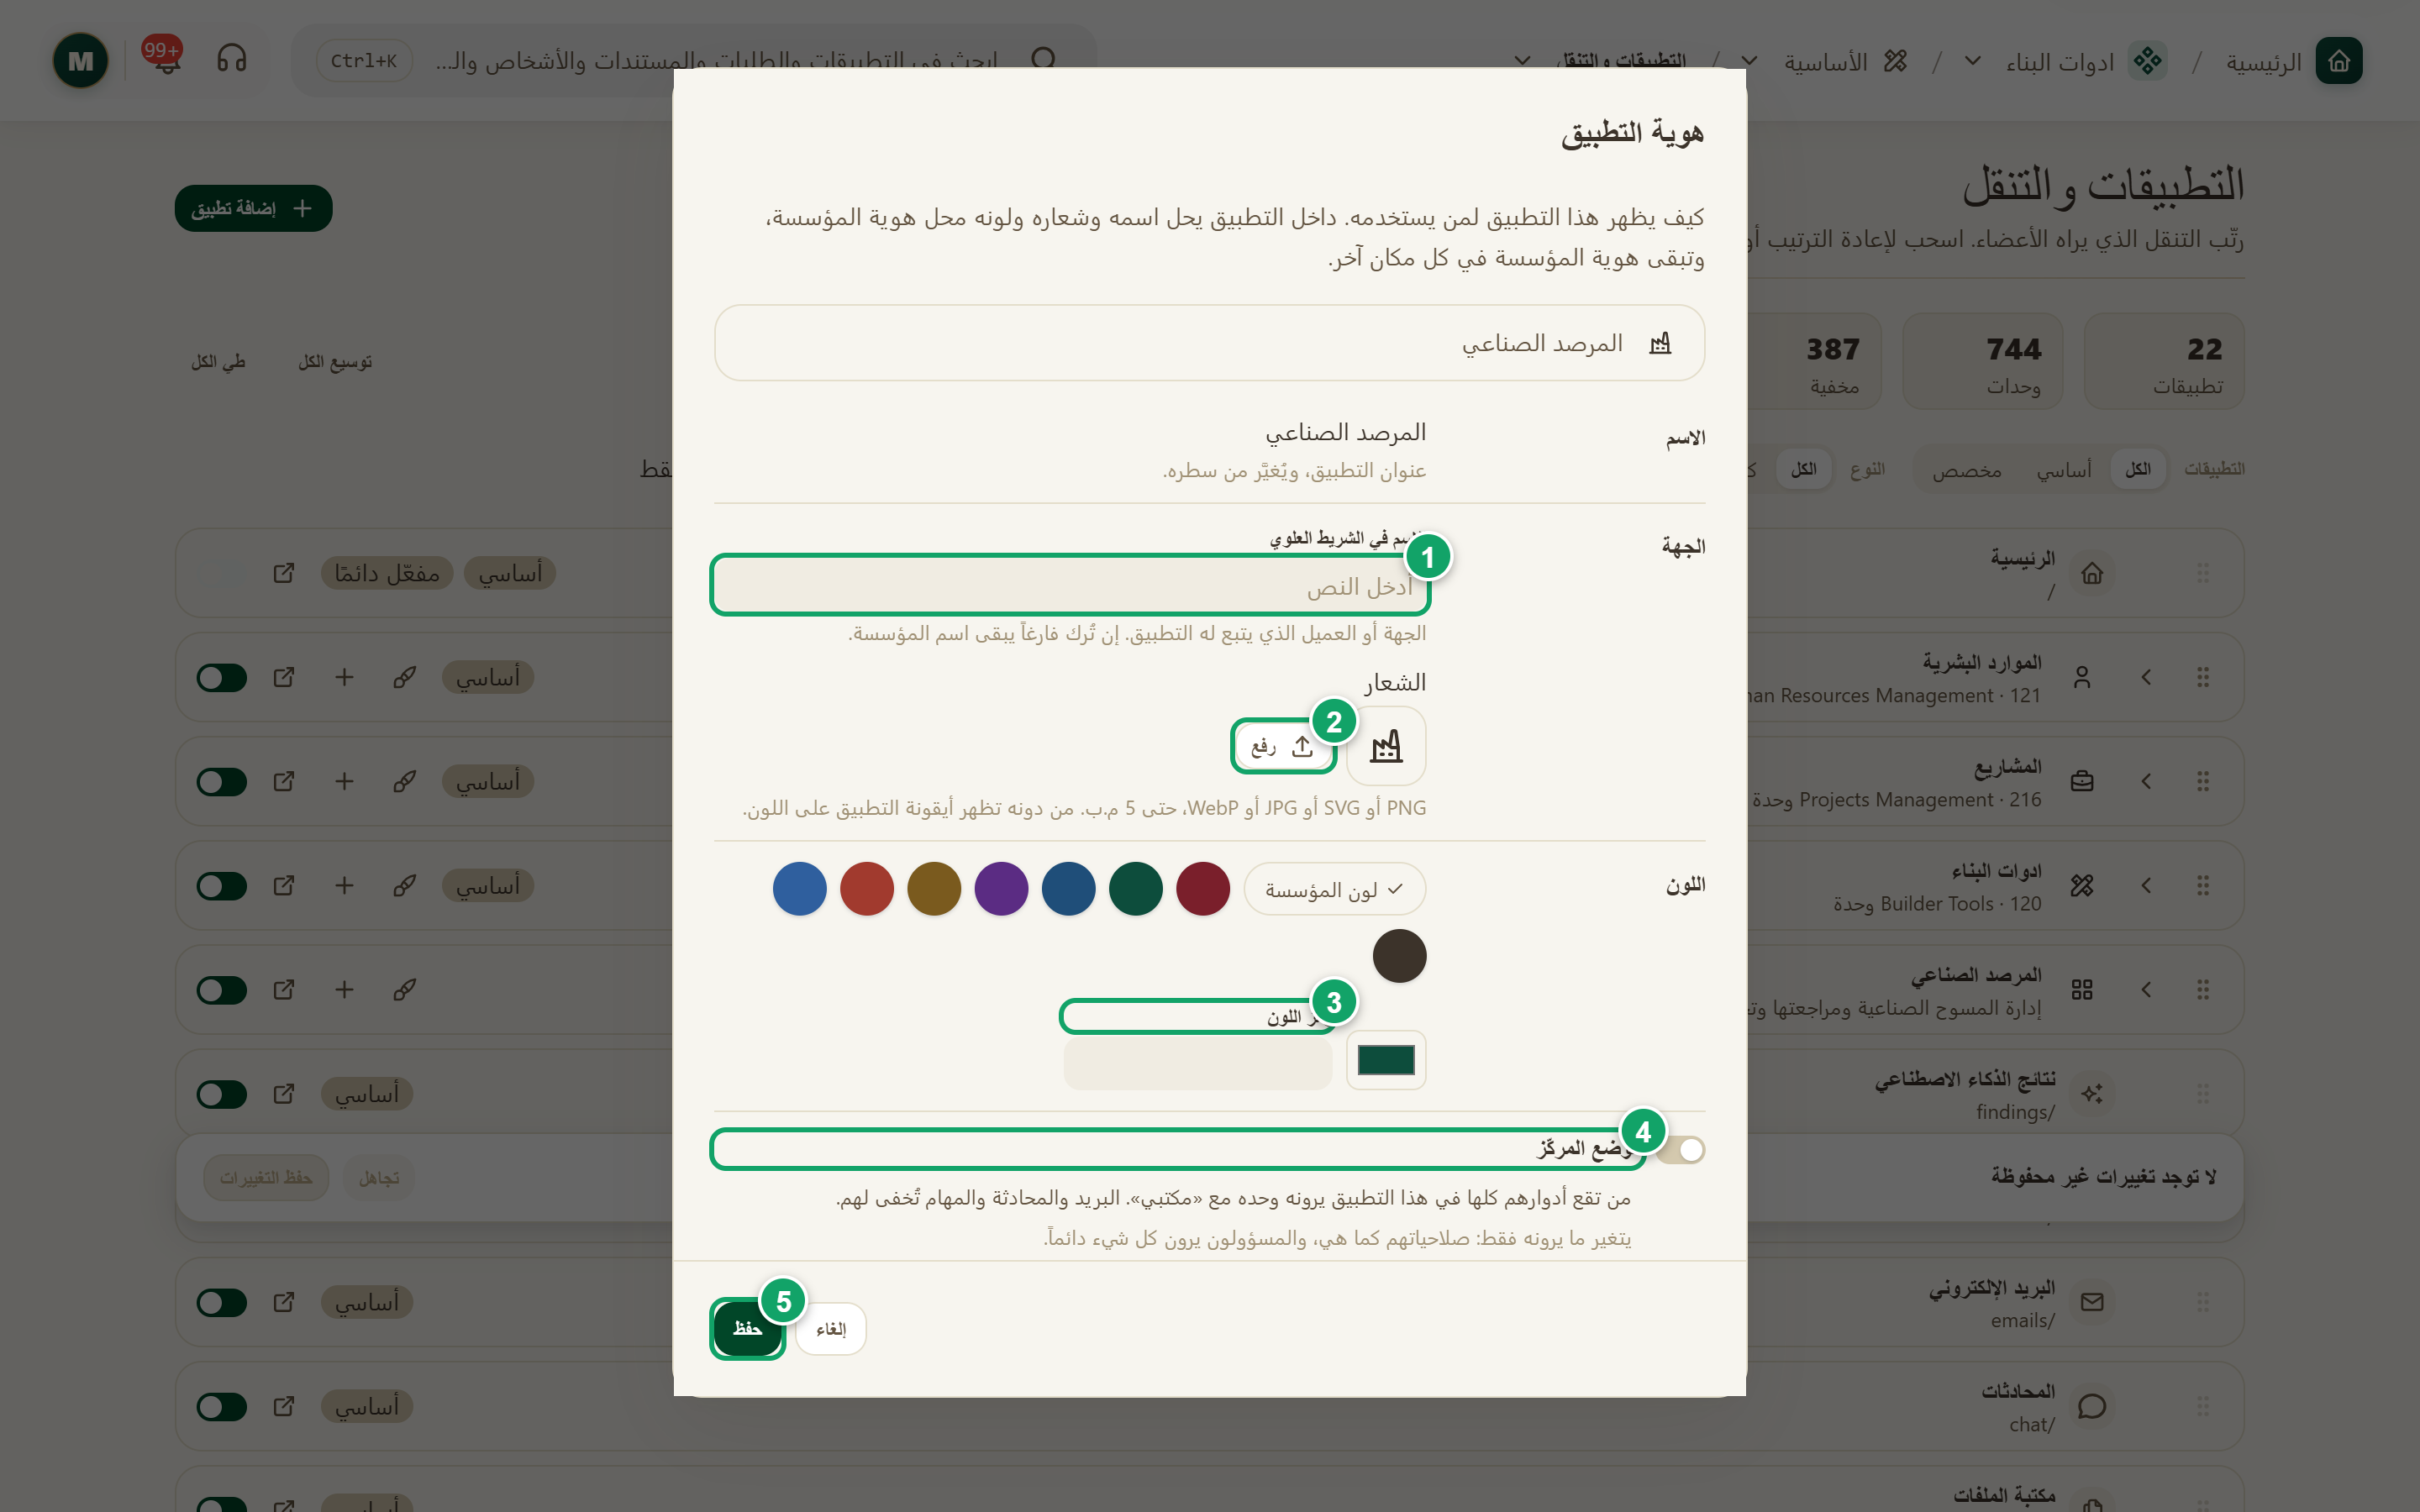
\includegraphics[width=0.95\linewidth,height=0.72\textheight,keepaspectratio]{figures/screens/ch06-nav-identity-ar.png}
\caption{نافذة «هوية التطبيق»}
\label{fig:builder-navigation-identity-screen}
\shotnote{تعرض الصورة نافذة «هوية التطبيق» لتطبيق «المرصد الصناعي» في مؤسسة الاختبار قبل أي تعديل، وتبدأ بمعاينة تتغير مع كل اختيار. وتجمع النافذة الاسم والشعار واللون والوضع المركّز، ثم تحفظها معاً دون الحاجة إلى «حفظ التغييرات». ① «الاسم في الشريط العلوي»: اسم الجهة التي يتبعها التطبيق. ② «رفع»: يرفع صورة الشعار. ③ «رمز اللون»: لون مخصص بالصيغة \en{\#RRGGBB}، ويمكنك بدلاً منه اختيار أحد الألوان الجاهزة. ④ «الوضع المركّز»: يقصر ما يراه أعضاء التطبيق عليه وحده. ⑤ «حفظ»: يحفظ الهوية فوراً.}
\end{figure}

\begin{table}[H]
\centering
\caption{محتوى نافذة «هوية التطبيق»}
\label{tab:builder-navigation-identity-fields}
\begin{tabularx}{\linewidth}{R{3.6cm} Y}
\rcHeaderRow
\thh{الجزء} & \thh{ما يحدده}\\
معاينة & تعرض الشعار واللون والاسم معاً كما ستظهر في الشريط العلوي، وتتغير مع كل اختيار.\\
الاسم & عنوان التطبيق للعرض فقط، ولا يُعدَّل من هذه النافذة.\\
الاسم في الشريط العلوي & اسم الجهة أو العميل الذي يتبع له التطبيق، بكل لغة. وإذا تُرك فارغاً يبقى اسم المؤسسة.\\
الشعار & صورة بصيغة \en{PNG} أو \en{SVG} أو \en{JPG} أو \en{WebP} لا يتجاوز حجمها 5 ميغابايت، ترفعها بزر «رفع» وتغيّرها بزر «استبدال» أو تحذفها بزر «إزالة». ومن دونها تظهر أيقونة التطبيق على اللون.\\
اللون & «لون المؤسسة»، أو أحد ثمانية ألوان جاهزة، أو «لون مخصص» تختاره أو تكتب «رمز اللون» بالصيغة \en{\#RRGGBB}. ويظهر تحذير إذا صعبت قراءة النص الأبيض على اللون.\\
الوضع المركّز & من تقع أدوارهم كلها داخل هذا التطبيق يرونه وحده مع «مكتبي»، ويُخفى عنهم البريد والمحادثة والمهام. ولا تتغير صلاحياتهم، ويرى المسؤولون كل شيء دائماً.\\
يبقى لهم & يظهر عند تشغيل الوضع المركّز، وتختار منه ما يبقى ظاهراً لهؤلاء الأعضاء: «المهام» و«التقويم» و«البريد» و«المحادثة» و«المكتبة» و«ردود النماذج» و«الموارد البشرية» و«المشاريع».\\
\end{tabularx}
\end{table}

\begin{rcwarn}[الوضع المركّز يغيّر ما يُعرض فقط]
لا يمنح الوضع المركّز صلاحية ولا يسحبها، بل يخفي التطبيقات الأخرى عن الأعضاء الذين تقع أدوارهم كلها في هذا التطبيق. فإذا كان لعضو دور في تطبيق آخر، فلن يتأثر بهذا الوضع. ويظهر بجانب التطبيق في الشجرة شارة «مركّز» ما دام الوضع مفعّلاً.
\end{rcwarn}

\begin{figure}[H]
\centering
\begin{tikzpicture}[node distance=0.5cm]
\node[stepBox] (a) {\RL{زر هوية التطبيق}};
\node[stepBox,below=of a] (b) {\RL{الاسم في الشريط العلوي}};
\node[stepBox,below=of b] (c) {\RL{الشعار واللون}};
\node[stepBox,below=of c] (d) {\RL{الوضع المركّز عند الحاجة}};
\node[stepBox,below=of d] (e) {\RL{مراجعة المعاينة ثم حفظ}};
\draw[flowsTo] (a) -- (b);
\draw[flowsTo] (b) -- (c);
\draw[flowsTo] (c) -- (d);
\draw[flowsTo] (d) -- (e);
\end{tikzpicture}
\rclegend
\caption{ضبط هوية التطبيق}
\label{fig:builder-navigation-identity-flow}
\shotnote{يتبع المخطط ترتيب أجزاء النافذة، ويضع المعاينة قبل الحفظ مباشرة لأنها تريك النتيجة كما ستظهر في الشريط العلوي. وخطوة الوضع المركّز اختيارية، فاتركها إذا كان أعضاء التطبيق يحتاجون إلى بقية التطبيقات في عملهم اليومي.}
\end{figure}

\subsection{خطوات العمل والتحقق}
\begin{enumerate}
\item افتح «التطبيقات والتنقل»، وابحث عن التطبيق، واضغط زر «هوية التطبيق» في صفه.
\item اكتب «الاسم في الشريط العلوي» إذا كان التطبيق يتبع جهة غير المؤسسة.
\item ارفع شعاراً بزر «رفع» إن وُجد، واختر لوناً جاهزاً أو اكتب «رمز اللون».
\item شغّل «الوضع المركّز» إذا أردت أن يرى أعضاء التطبيق هذا التطبيق وحده، واختر من «يبقى لهم» ما يحتاجون إليه.
\item راجع «معاينة»، ثم اضغط «حفظ».
\end{enumerate}

\textbf{تحقق ومعالجة المشكلة:} يجب أن تظهر رسالة «حُفظت هوية التطبيق.»، وأن تظهر الهوية في الشريط العلوي عند فتح التطبيق. فإذا بقي «حفظ» معطلاً، فصحّح «رمز اللون» ليكون بالصيغة \en{\#RRGGBB} أو أفرغ الحقل. وإذا ظهرت «حجم الشعار أكبر من 5 م.ب.»، فصغّر الصورة ثم ارفعها مرة أخرى.

\clearpage
\section{إضافة طريقة عرض إلى القائمة}
\label{sec:builder-feature-navigation-views}

طريقة العرض المحفوظة هي قائمة سجلات بتصفية وترتيب جاهزين، مثل «الطلبات التي تنتظر المراجعة». ويمكنك أن تضعها عنصراً مستقلاً في قسم من القائمة، فيفتحها العضو مباشرة دون أن يفتح القائمة الكاملة ثم يختار التصفية. ويمكن أن يظهر بجانبها عدد السجلات الحالي، فيعرف العضو حجم العمل قبل أن يفتحها.

وتُضاف طريقة العرض مسودةً، ولا يراها الأعضاء حتى تشغّل مفتاحها في الشجرة وتحفظ التغييرات.

\textbf{المسار ومن يستخدمه:} «ادوات البناء» ← «الأساسية» ← «التطبيقات والتنقل» ← زر «إضافة طريقة عرض إلى…» في صف القسم. يظهر الزر عندما تكون ميزة «طرق العرض في القوائم» مفعّلة في «التنقل حسب العمل»، وللأقسام التي لها سجل فقط.

\begin{rcnote}[مثال: شركة الأفق]
يضيف مسؤول النظام إلى قسم «الزيارات» طريقة العرض المحفوظة «بانتظار المراجعة» من «طلبات الزيارة»، ويشغّل «إظهار العدد الحالي» بلون «تنبيه». وبعد نشرها ترى سارة الخطيب عدد الطلبات التي تنتظرها بجانب اسمها في القائمة. ويختار النوع من ① ويشغّل العدد من ③ ويختار لونه من ④.
\end{rcnote}

\begin{figure}[H]
\centering
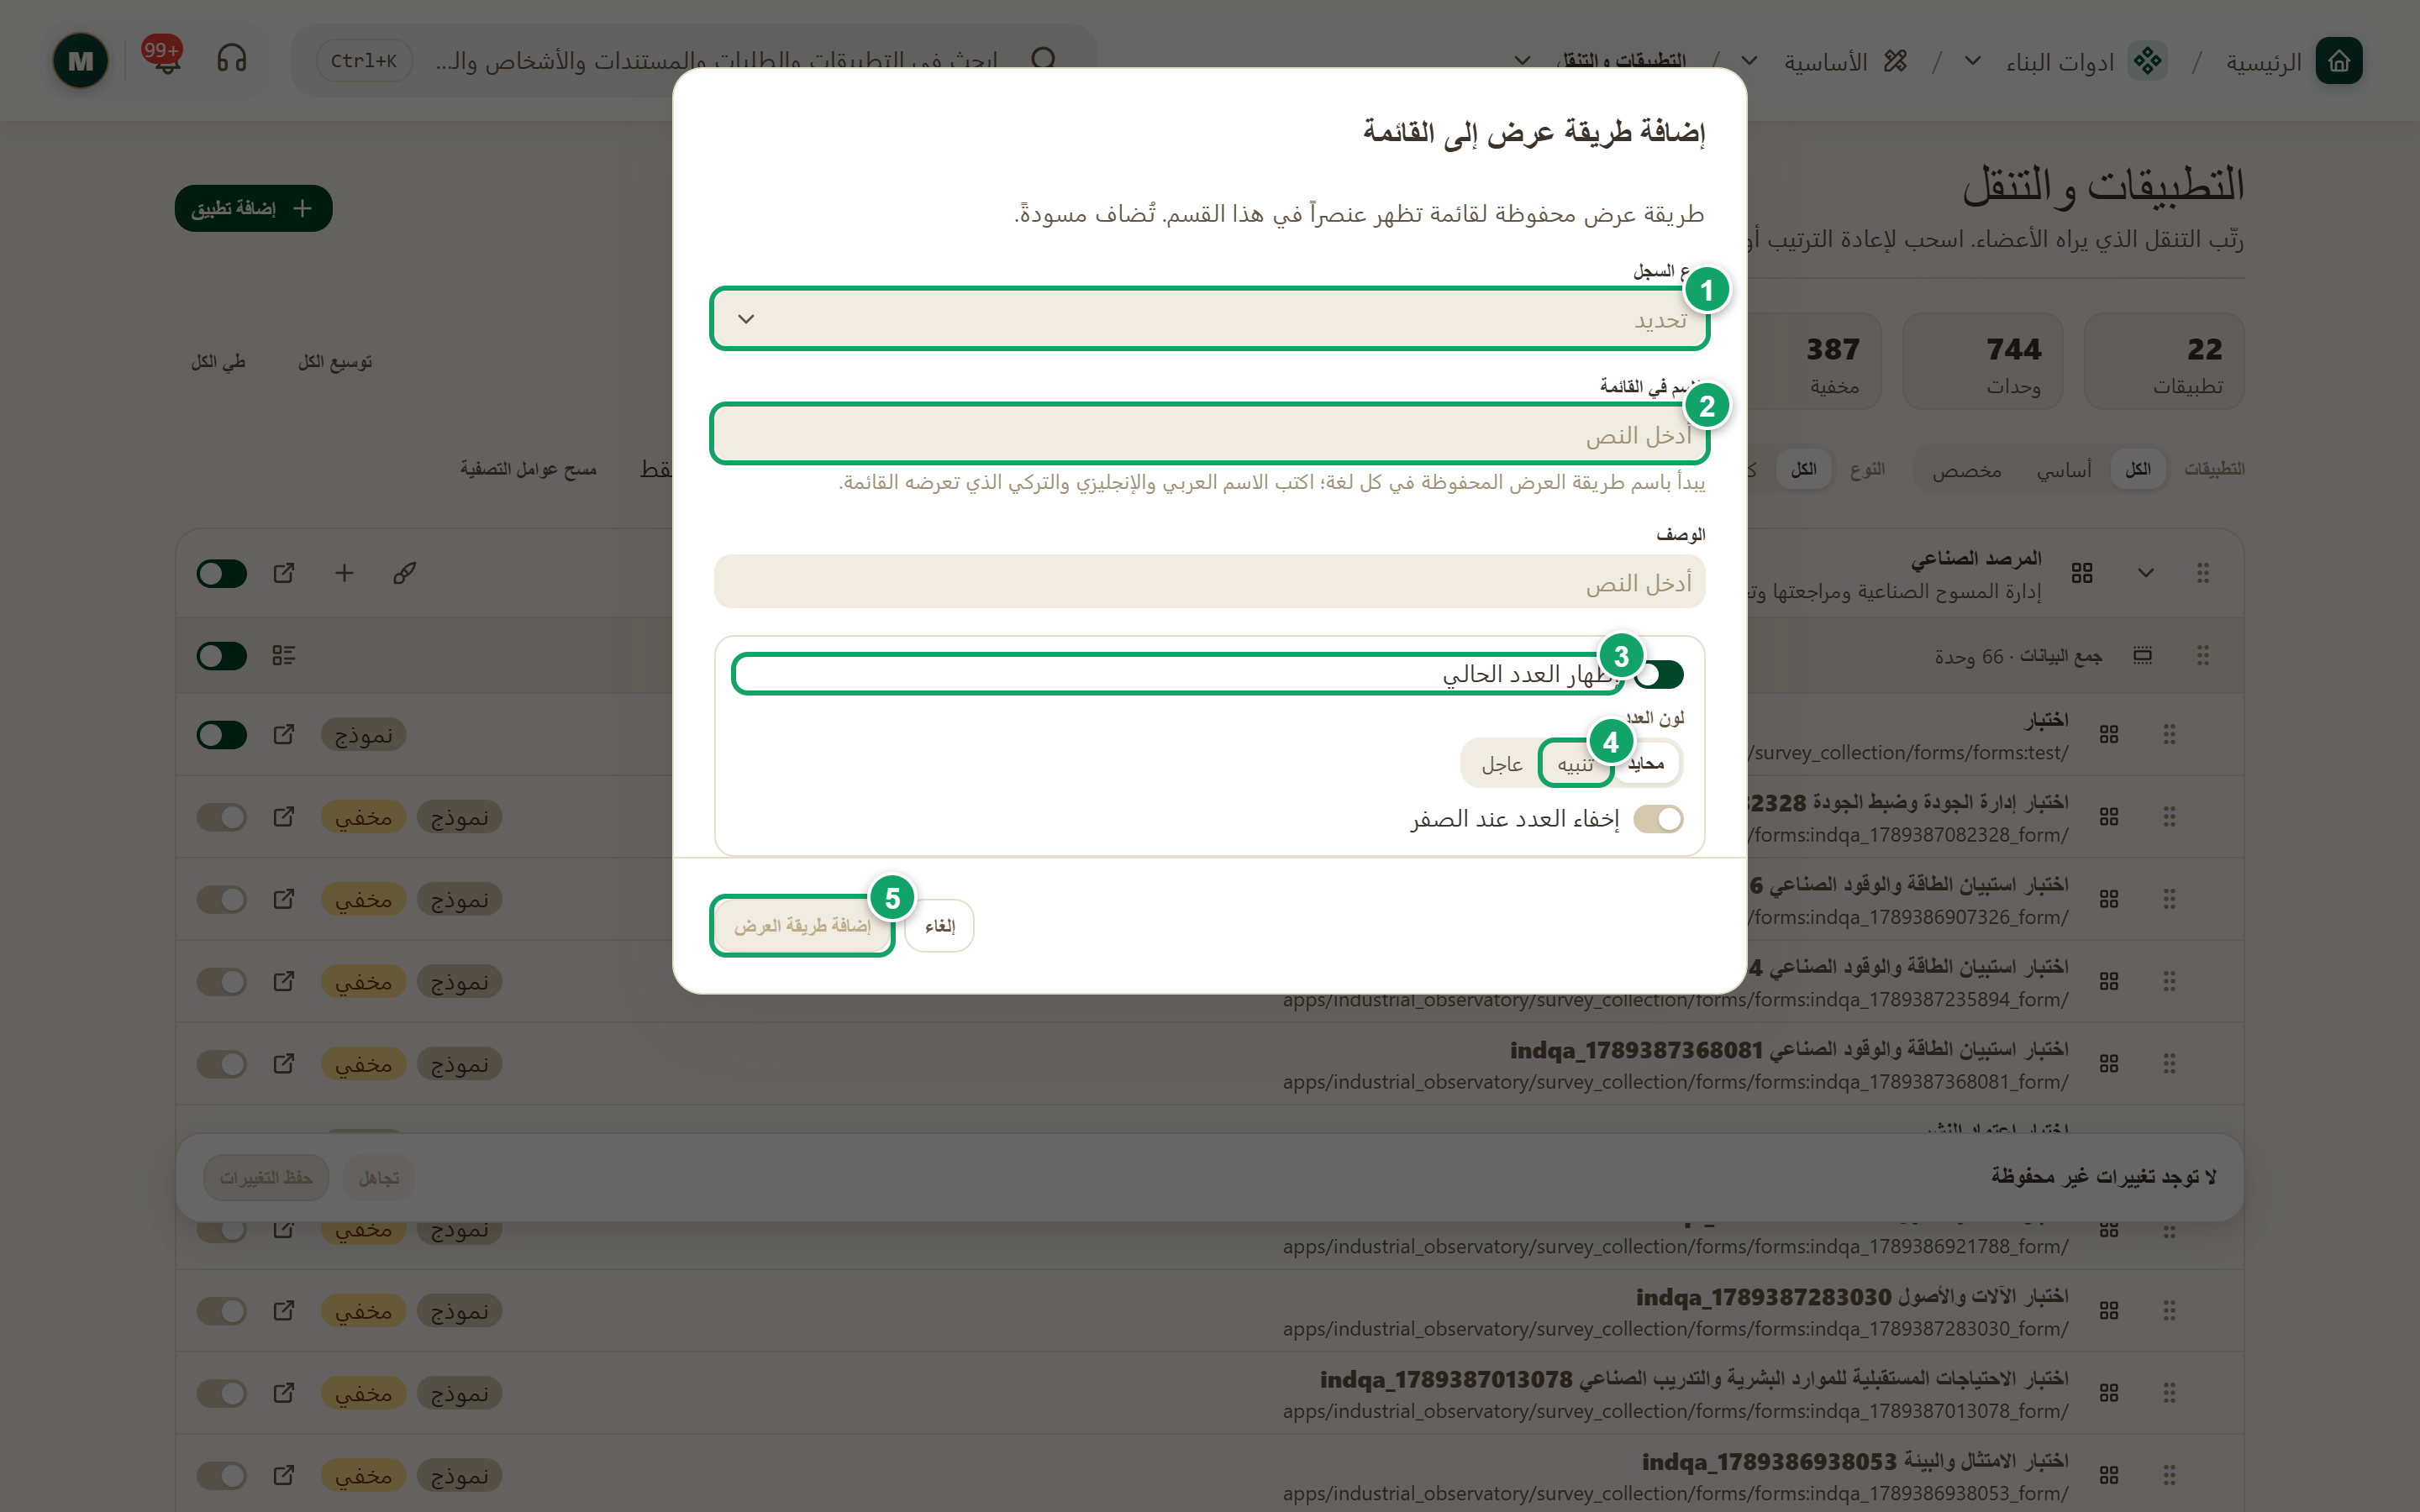
\includegraphics[width=0.95\linewidth,height=0.72\textheight,keepaspectratio]{figures/screens/ch06-nav-add-view-ar.png}
\caption{نافذة «إضافة طريقة عرض إلى القائمة»}
\label{fig:builder-navigation-views-screen}
\shotnote{تعرض الصورة النافذة بعد الضغط على زر الإضافة في صف قسم «جمع البيانات» من مؤسسة الاختبار، وقبل اختيار نوع السجل الذي تعتمد عليه قائمة طرق العرض المحفوظة. ويظهر فيها «إظهار العدد الحالي» مشغّلاً افتراضياً، والعنصر الذي تضيفه يبقى مسودة حتى تنشره من الشجرة. ① «نوع السجل»: النوع الذي تأتي منه طريقة العرض. ② «الاسم في القائمة»: الاسم الذي يراه الأعضاء. ③ «إظهار العدد الحالي»: يعرض عدد السجلات بجانب الاسم. ④ «تنبيه»: أحد ألوان العدد. ⑤ «إضافة طريقة العرض»: يضيف العنصر إلى القسم مسودةً.}
\end{figure}

\begin{table}[H]
\centering
\caption{حقول نافذة «إضافة طريقة عرض إلى القائمة»}
\label{tab:builder-navigation-views-fields}
\begin{tabularx}{\linewidth}{R{3.6cm} Y}
\rcHeaderRow
\thh{الحقل} & \thh{ما تختاره}\\
نوع السجل & نوع السجلات الذي تأتي منه طريقة العرض. وتظهر هنا الأنواع التي بنتها المؤسسة، لا الأنواع المضمّنة في النظام.\\
طريقة العرض المحفوظة & إحدى طرق العرض المشتركة لهذا النوع. وإذا لم تكن له أي طريقة مشتركة، تطلب منك النافذة إضافتها أولاً من «القوائم وطرق العرض» في المنشئ.\\
الاسم في القائمة & يبدأ باسم طريقة العرض، ويمكنك تغييره بالعربية والإنجليزية والتركية.\\
الوصف & شرح قصير اختياري لما تعرضه.\\
العرض بشكل & «كما حُفظت طريقة العرض»، أو شكل آخر متاح للنوع، مثل الجدول أو اللوحة.\\
إظهار العدد الحالي & يعرض عدد السجلات بجانب الاسم، مع «لون العدد»: «محايد» أو «تنبيه» أو «عاجل»، ومع خيار «إخفاء العدد عند الصفر».\\
\end{tabularx}
\end{table}

\subsection{بعد الإضافة}

يظهر العنصر الجديد في القسم بشارة «طريقة عرض» وشارة «مسودة». فإذا شغّلت مفتاحه وضغطت «حفظ التغييرات»، يُنشر ويظهر للأعضاء. ولتعديل اسمه أو عدده لاحقاً، اضغط زر «تعديل» في صفه، فتفتح نافذة «تعديل طريقة العرض في القائمة»؛ والحفظ فيها يُبقي العنصر منشوراً أو مسودة كما كان.

\begin{figure}[H]
\centering
\begin{tikzpicture}[node distance=0.5cm]
\node[stepBox] (a) {\RL{تفعيل طرق العرض في القوائم}};
\node[stepBox,below=of a] (b) {\RL{إضافة طريقة عرض في صف القسم}};
\node[stepBox,below=of b] (c) {\RL{نوع السجل وطريقة العرض}};
\node[stepBox,below=of c] (d) {\RL{الاسم والعدد}};
\node[stepBox,below=of d] (e) {\RL{تشغيل المفتاح وحفظ التغييرات}};
\draw[flowsTo] (a) -- (b);
\draw[flowsTo] (b) -- (c);
\draw[flowsTo] (c) -- (d);
\draw[flowsTo] (d) -- (e);
\end{tikzpicture}
\rclegend
\caption{من طريقة عرض محفوظة إلى عنصر في القائمة}
\label{fig:builder-navigation-views-flow}
\shotnote{يبدأ المخطط من صفحة «التنقل حسب العمل» لأن زر الإضافة لا يظهر قبل تفعيل الميزة فيها. وينتهي بتشغيل المفتاح والحفظ، لأن الإضافة تُنشئ مسودة فقط، ولا يرى الأعضاء العنصر قبل نشره.}
\end{figure}

\subsection{خطوات العمل والتحقق}
\begin{enumerate}
\item تأكد من أن «طرق العرض في القوائم» مفعّلة ومحفوظة في «التنقل حسب العمل».
\item افتح «التطبيقات والتنقل»، ووسّع التطبيق، واضغط زر إضافة طريقة العرض في صف القسم.
\item اختر «نوع السجل» ثم «طريقة العرض المحفوظة»، وراجع «الاسم في القائمة».
\item شغّل «إظهار العدد الحالي» إذا أردته، واختر «لون العدد»، ثم اضغط «إضافة طريقة العرض».
\item شغّل مفتاح العنصر الجديد في القسم، واضغط «حفظ التغييرات».
\end{enumerate}

\textbf{تحقق ومعالجة المشكلة:} بعد الإضافة تظهر رسالة «أُضيفت طريقة العرض إلى … مسودةً» باسم القسم، وبعد الحفظ تختفي عن العنصر شارة «مسودة». فإذا لم يظهر زر الإضافة، ففعّل الميزة واحفظها في «التنقل حسب العمل» ثم أعد تحميل الصفحة. وإذا لم تجد طريقة العرض في القائمة المنسدلة، فاجعلها مشتركة من «القوائم وطرق العرض» في المنشئ وانشر النوع.

\clearpage
\section{التنقل حسب العمل}
\label{sec:builder-feature-work-navigation}

تحدد هذه الصفحة ما يراه كل عضو أولاً عندما يبدأ يومه، دون أن تُنشئ بيانات جديدة. فهي تجمع العمل الموجود في أماكن أقرب إليه: قائمة «المستحق عليّ» التي تعرض ما ينتظره، وسياقاً مشتركاً مثل السنة أو الدورة تتبعه القوائم واللوحات، وطرق عرض محفوظة تظهر في القوائم بعدّاداتها.

وتتوزع الإعدادات على أربعة تبويبات: «الميزات» و«المصادر» و«السياق» و«اللوحات». وهي كلها مسودة واحدة تُحفظ معاً بزر «حفظ». وكل ميزة متوقفة حتى تشغّلها، والمؤسسة التي لا تشغّل أي ميزة تعمل كما كانت تماماً.

\textbf{المسار ومن يستخدمه:} «ادوات البناء» ← «الأساسية» ← «التنقل حسب العمل». تظهر لمالك المؤسسة ومسؤولها فقط.

\begin{rcnote}[مثال: شركة الأفق]
يفعّل مسؤول النظام «قائمة المستحق عليّ»، ويضيف إليها طلبات الزيارة التي تنتظر قرار سارة الخطيب، فتجدها سارة في مكان واحد كل صباح بدلاً من فتح كل قائمة على حدة. ويشغّل الميزة من ② في تبويب ①، ثم يضيف المصدر من ③ ويحفظ من ④.
\end{rcnote}

\begin{figure}[H]
\centering
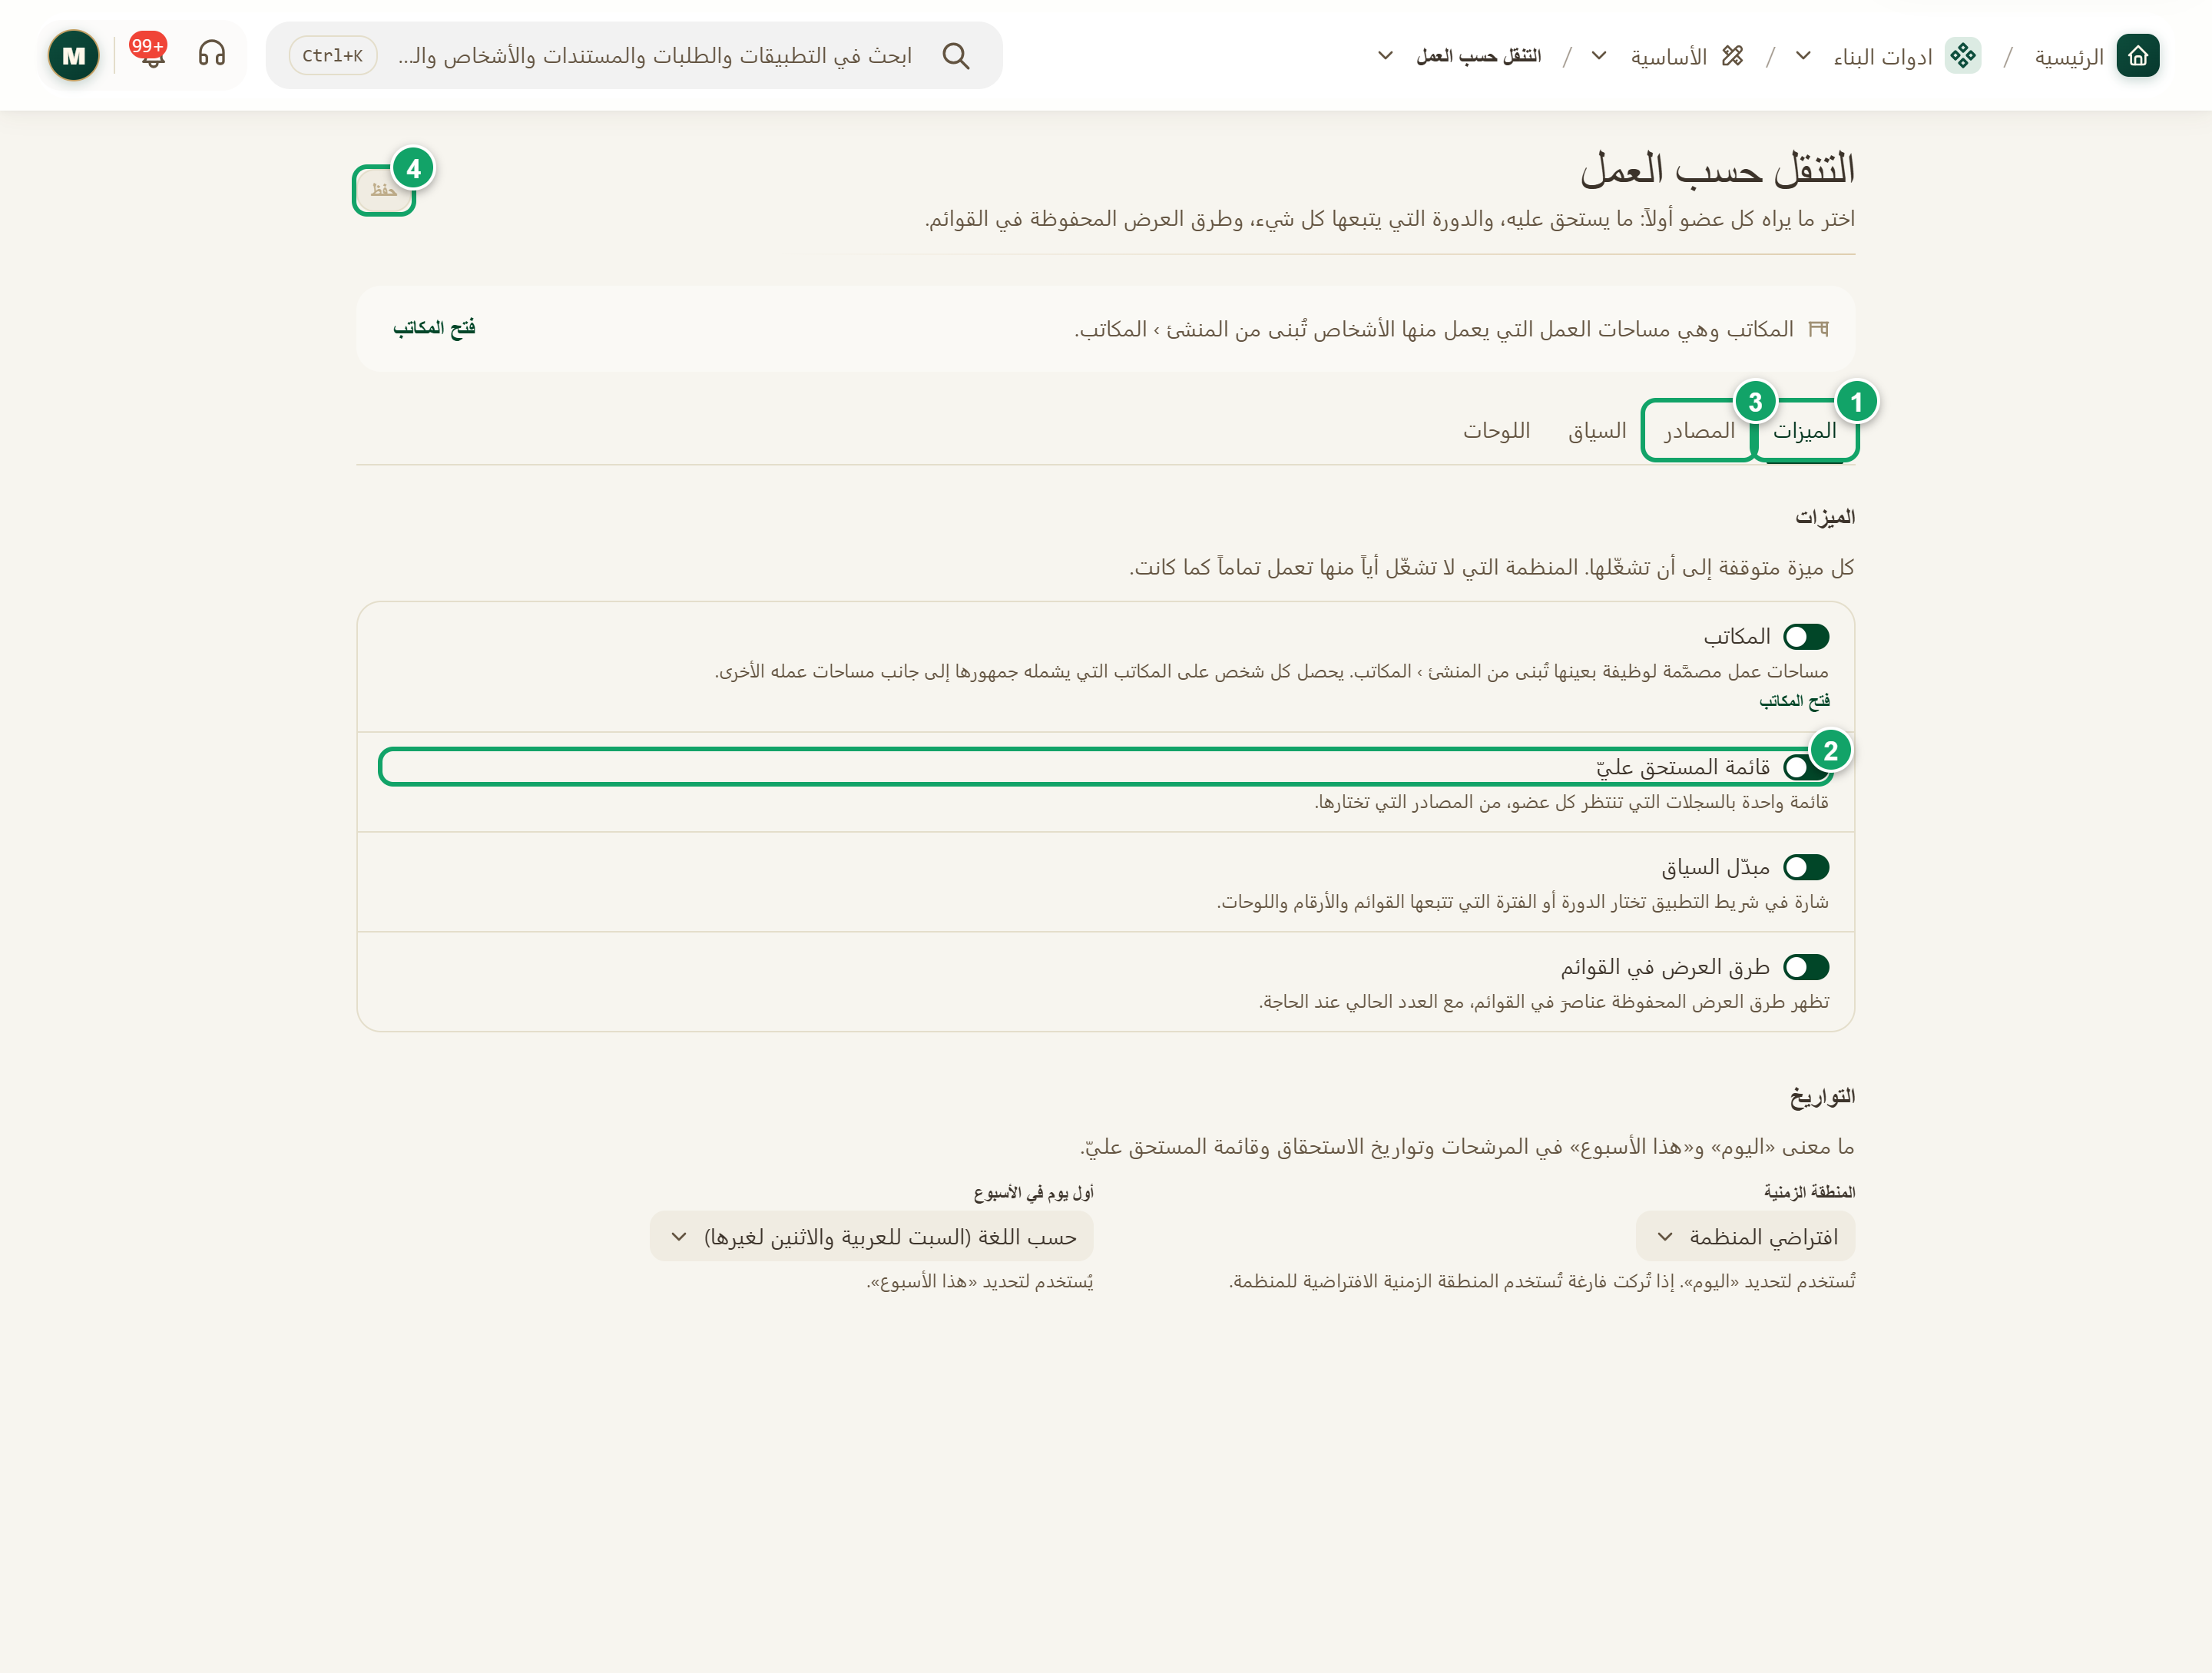
\includegraphics[width=0.95\linewidth,height=0.72\textheight,keepaspectratio]{figures/screens/ch06-work-navigation-ar.png}
\caption{صفحة «التنقل حسب العمل»}
\label{fig:builder-work-navigation-screen}
\shotnote{تعرض الصورة تبويب «الميزات» في مؤسسة الاختبار، وقد شُغّلت فيه الميزات الأربع، أما في مؤسسة لم تضبط الصفحة فتبدأ كلها متوقفة. وتُحفظ التبويبات الأربعة معاً بزر واحد، لذلك راجع ما غيّرته فيها قبل الحفظ. ① «الميزات»: التبويب الذي تشغّل منه «المكاتب» و«قائمة المستحق عليّ» وغيرهما. ② مفتاح «قائمة المستحق عليّ»: يشغّل القائمة التي تجمع ما ينتظر العضو. ③ «المصادر»: يحدد ما يغذّي هذه القائمة. ④ «حفظ»: يحفظ الإعدادات، ويبقى معطلاً حتى تغيّر شيئاً.}
\end{figure}

\begin{table}[H]
\centering
\caption{تبويب «الميزات»}
\label{tab:builder-work-navigation-data}
\begin{tabularx}{\linewidth}{R{3.6cm} Y}
\rcHeaderRow
\thh{الإعداد} & \thh{ماذا يفعل؟}\\
المكاتب & يشغّل المكاتب، وهي مساحات عمل مصمَّمة لوظيفة بعينها. وتُبنى المكاتب في صفحة مستقلة تفتحها من رابط «فتح المكاتب».\\
قائمة المستحق عليّ & يجمع في قائمة واحدة السجلات التي تنتظر كل عضو، من المصادر التي تضيفها في تبويب «المصادر».\\
مبدّل السياق & يُظهر شريحة في شريط التطبيق يختار منها العضو الدورة أو الفترة التي تتبعها القوائم والأرقام واللوحات.\\
طرق العرض في القوائم & يتيح وضع طرق العرض المحفوظة عناصرَ في القوائم، مع عددها الحالي عند الحاجة.\\
التواريخ & «المنطقة الزمنية» التي يُحسب بها «اليوم»، و«أول يوم في الأسبوع» الذي يُحسب به «هذا الأسبوع»، في التصفية وتواريخ الاستحقاق وقائمة المستحق.\\
\end{tabularx}
\end{table}

\begin{table}[H]
\centering
\caption{بقية التبويبات}
\label{tab:builder-work-navigation-tabs}
\begin{tabularx}{\linewidth}{R{3.6cm} Y}
\rcHeaderRow
\thh{التبويب} & \thh{ماذا تحدد فيه؟}\\
المصادر & ما يغذّي قائمة «المستحق عليّ». ويشرحه قسم «مصادر قائمة المستحق عليّ».\\
السياق & نوع السجلات الذي تتبعه التطبيقات والأقسام المختارة. ويشرحه قسم «السياق».\\
اللوحات & نطاق بيانات اللوحات الجديدة، والانتقال باللوحات القديمة إلى صلاحيات المشاهد. ويشرحه قسم «نطاق بيانات اللوحات».\\
\end{tabularx}
\end{table}

\begin{figure}[H]
\centering
\begin{tikzpicture}[node distance=0.5cm]
\node[entity] (member) {\RL{العضو}};
\node[entityOpt,below right=0.7cm and 0.3cm of member] (desk) {\RL{المكاتب}};
\node[entityOpt,below left=0.7cm and 0.3cm of member] (due) {\RL{المستحق عليّ}};
\draw[dependsOnOpt] (member.south) -- ++(0,-0.3) -| (desk.north);
\draw[dependsOnOpt] (member.south) -- ++(0,-0.3) -| (due.north);
\end{tikzpicture}
\rclegend
\caption{ما يراه العضو أولاً}
\label{fig:builder-work-navigation-model}
\shotnote{يوضّح الشكل أن هذه الصفحة لا تُنشئ بيانات جديدة، بل تقرّب العمل الموجود من العضو: مكاتب تناسب وظيفته، وقائمة تجمع ما يستحق عليه من أنواع سجلات مختلفة. وكلاهما اختياري، لذلك فعّل ميزة واحدة وجرّبها قبل تفعيل غيرها.}
\end{figure}

\subsection{خطوات العمل والتحقق}
\begin{enumerate}
\item افتح «التنقل حسب العمل»، وشغّل في «الميزات» الميزة التي تحتاجها المؤسسة.
\item اختر «المنطقة الزمنية» و«أول يوم في الأسبوع» إذا كانت القيم الافتراضية لا تناسب المؤسسة.
\item إذا شغّلت «قائمة المستحق عليّ»، فانتقل إلى «المصادر» وأضف مصدراً واحداً على الأقل.
\item اضغط «حفظ» في رأس الصفحة، أو «تجاهل التغييرات» إذا أردت التراجع عن كل ما لم تحفظه.
\end{enumerate}

\textbf{تحقق ومعالجة المشكلة:} يجب أن تظهر رسالة «تم حفظ التنقل حسب العمل»، وأن يصبح زر «حفظ» معطلاً حتى تغيّر شيئاً آخر. فإذا ظهر تحت «قائمة المستحق عليّ» التنبيه «أضف مصدراً واحداً على الأقل في تبويب المصادر وإلا بقيت القائمة فارغة.»، فأضف مصدراً قبل أن تخبر الأعضاء بالميزة. وإذا ظهرت «إعدادات تحتاج إلى مراجعة» أو رسالة تعارض في الحفظ، فاتبع قسم «إعدادات تحتاج إلى مراجعة».

\clearpage
\section{مصادر قائمة المستحق عليّ}
\label{sec:builder-feature-work-navigation-sources}

قائمة «المستحق عليّ» فارغة في البداية، ولا يظهر فيها إلا ما تحدده المصادر. والمصدر قاعدة تقول: اعرض للعضو هذه السجلات لأنها تنتظره. وقد تكون السجلات التي يستطيع العضو تنفيذ انتقال عليها الآن، أو السجلات المسندة إليه في حقل عضو، أو قائمة مضمّنة في النظام مثل الموافقات.

ويضيف كل مصدر سجلاته إلى قوائم كل الأعضاء الذين تنطبق عليهم شروطه، ويمكن حصره في أدوار معينة. ولا يعطي المصدر أحداً صلاحية جديدة، فالعضو لا يرى إلا السجلات التي يستطيع فتحها.

\textbf{المسار ومن يستخدمه:} «ادوات البناء» ← «الأساسية» ← «التنقل حسب العمل» ← «المصادر». يستخدمه مالك المؤسسة ومسؤولها بعد تشغيل «قائمة المستحق عليّ».

\begin{rcnote}[مثال: شركة الأفق]
يضيف مسؤول النظام مصدراً من نوع «انتقالات أستطيع تنفيذها» باسم «زيارات بانتظار القرار»، ويختار «طلبات الزيارة» وحقل حالتها وانتقال الاعتماد. فتظهر الطلبات في قائمة سارة الخطيب لأنها تملك صلاحية الاعتماد، ولا تظهر لعمر حداد. ويضيف المصدر من ② ويحفظ من ③، ثم يتحقق منه من ④.
\end{rcnote}

\begin{figure}[H]
\centering
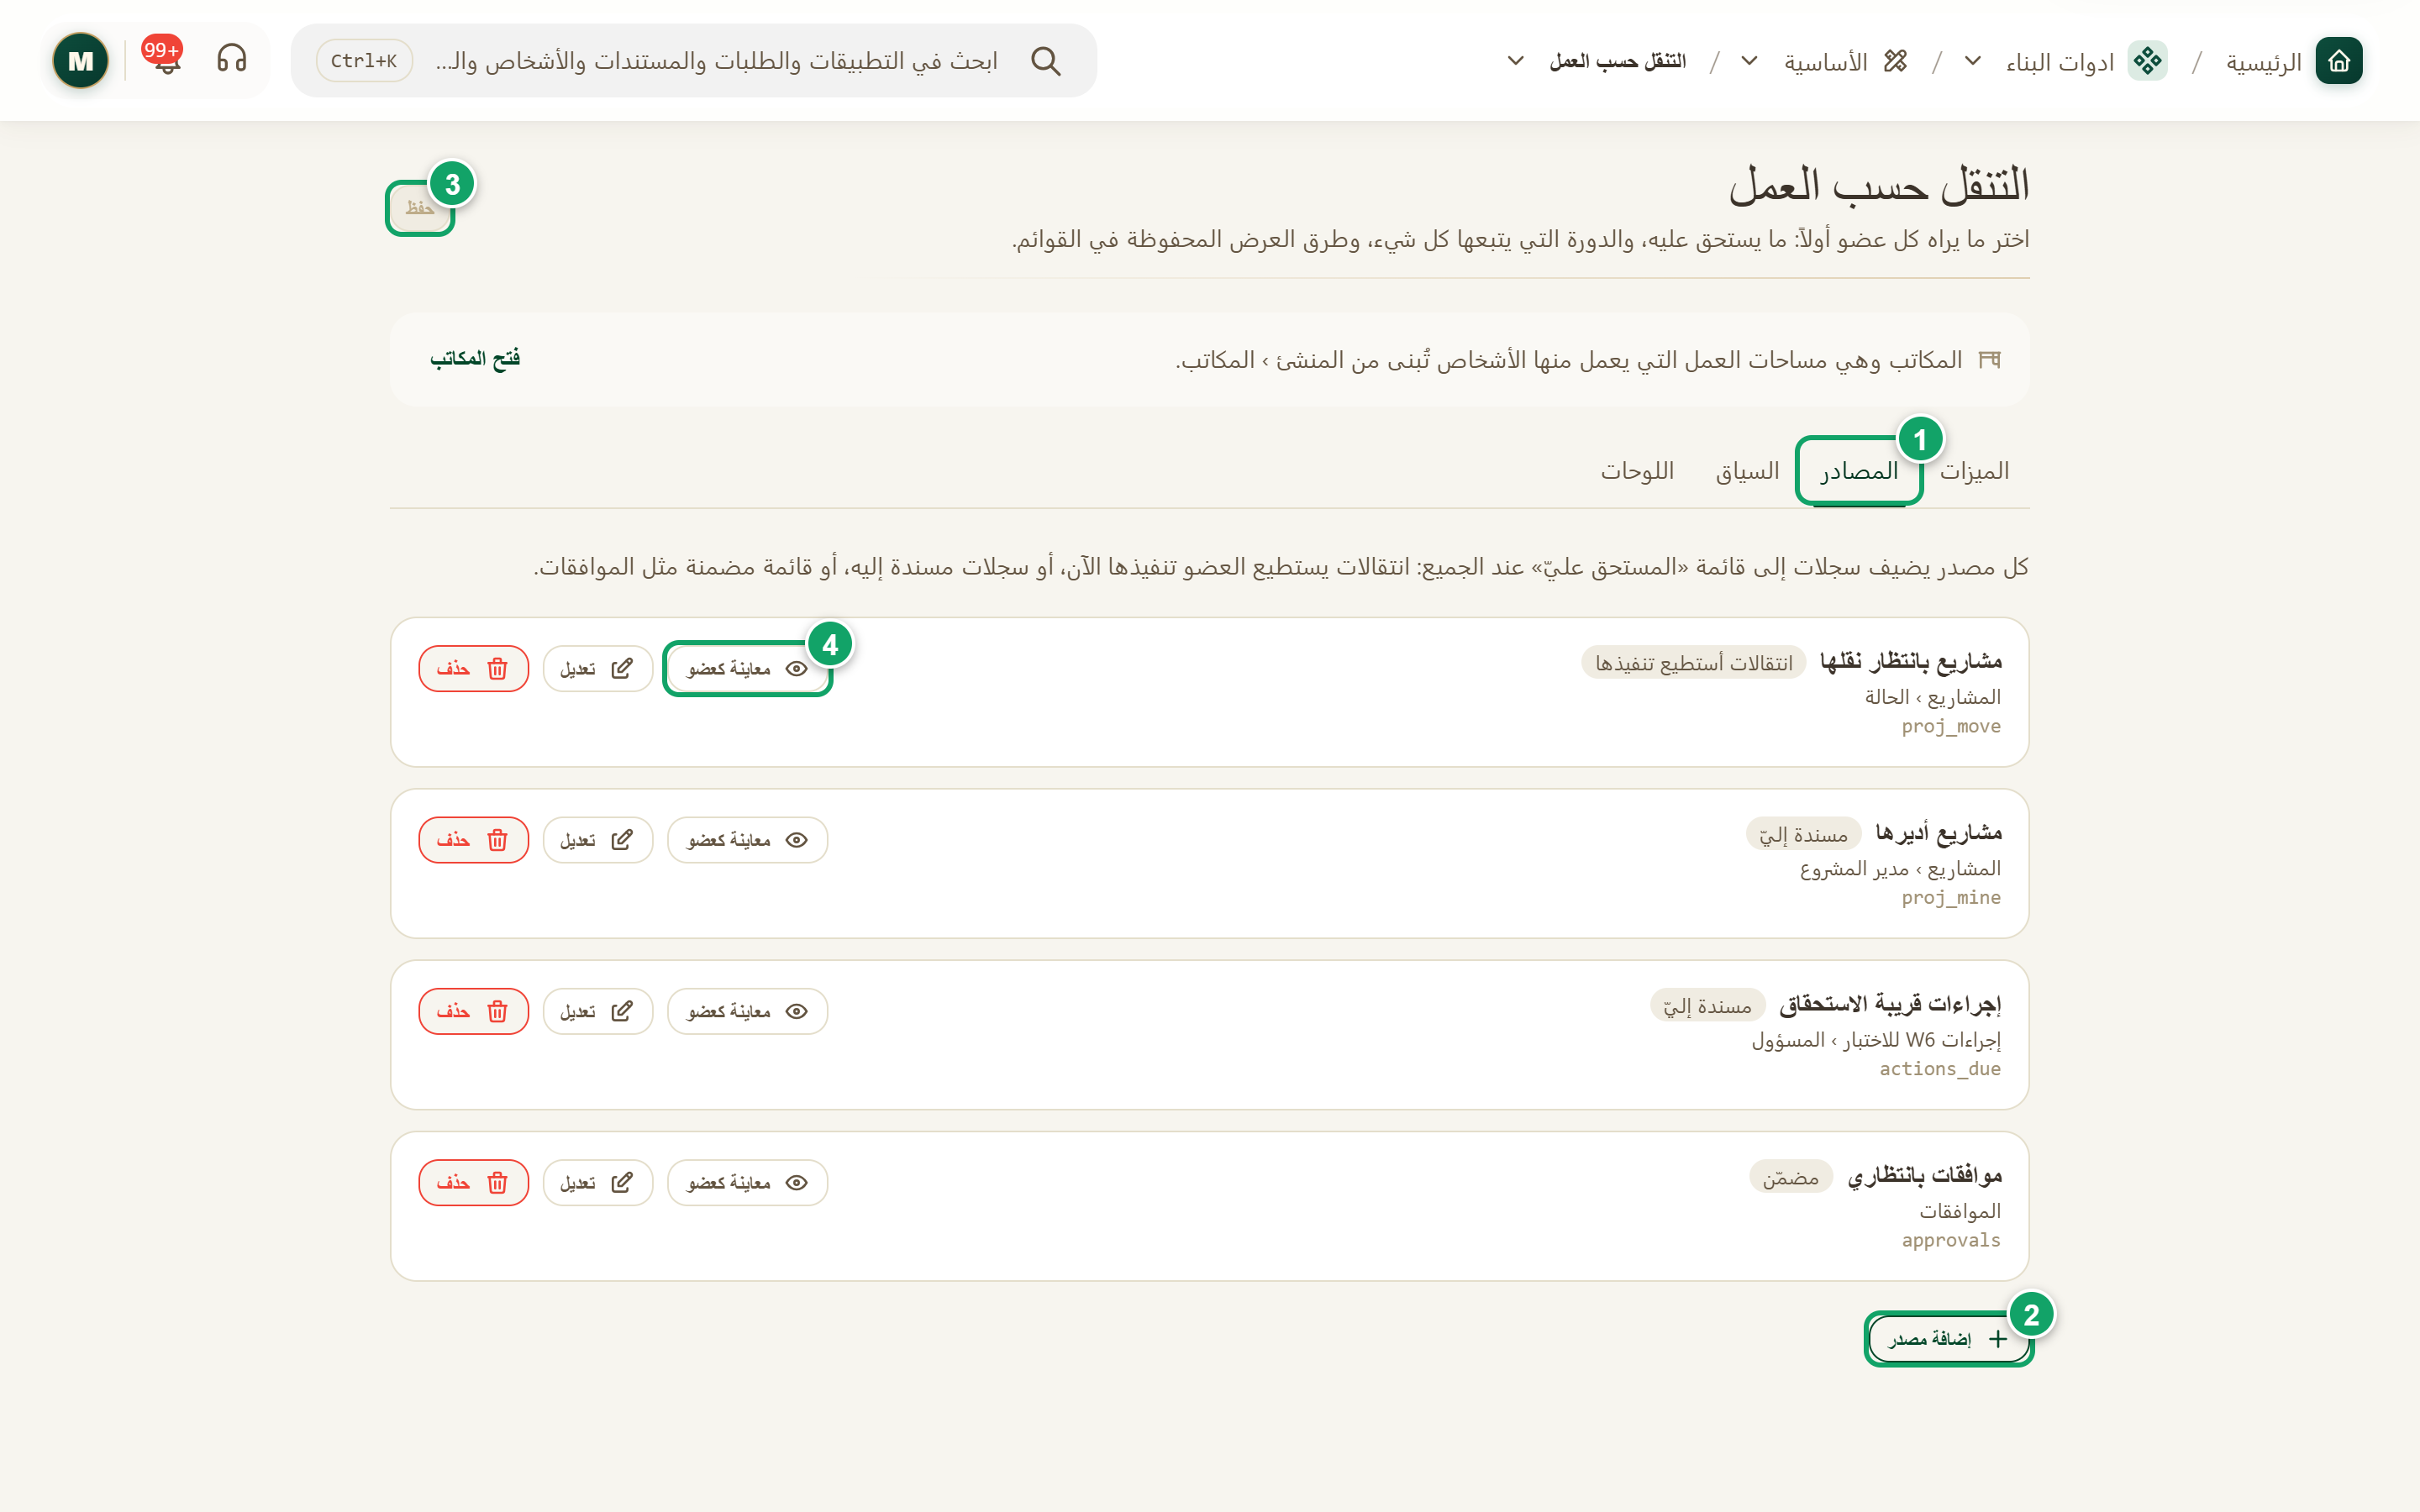
\includegraphics[width=0.95\linewidth,height=0.72\textheight,keepaspectratio]{figures/screens/ch06-wn-sources-ar.png}
\caption{تبويب «المصادر»}
\label{fig:builder-work-navigation-sources-screen}
\shotnote{تعرض الصورة تبويب «المصادر» في مؤسسة الاختبار، وفيه أربعة مصادر من الأنواع الثلاثة، يحمل كل منها شارة نوعه ونوع السجل الذي يقرؤه ومفتاحه. ويفيدك ذلك في مقارنة المصادر الموجودة قبل أن تضيف مصدراً جديداً. ① «المصادر»: التبويب الذي يعرض المصادر. ② «إضافة مصدر»: يفتح نافذة المصدر الجديد. ③ «حفظ»: يحفظ المصادر مع بقية إعدادات الصفحة. ④ «معاينة كعضو»: يعرض عدد السجلات وأمثلة منها بعد الحفظ.}
\end{figure}

\begin{table}[H]
\centering
\caption{أنواع المصادر}
\label{tab:builder-work-navigation-sources-kinds}
\begin{tabularx}{\linewidth}{R{3.6cm} Y}
\rcHeaderRow
\thh{النوع} & \thh{ما يجلبه وما تحدده}\\
انتقالات أستطيع تنفيذها & سجلات يستطيع العضو تنفيذ انتقال عليها الآن، مثل الاعتماد أو المراجعة. تختار «نوع السجل» و«حقل الحالة» و«الانتقالات التي تُعد عملاً»، وإذا تركتها فارغة شملت كل الانتقالات عدا التعديل العادي.\\
مسندة إليّ & سجلات يذكر فيها أحد «حقول العضو» هذا العضو. ويمكنك تحديد «ما الحالات المفتوحة»: «أي حالة» أو «حسب الفئة» أو «حالات محددة»، وتحديد فترة بحقلي «يبدأ في (حقل)» و«ينتهي في (حقل)».\\
مضمّن & قائمة جاهزة تختارها من «القائمة المضمنة»، مثل «الموافقات» و«موافقات الإجراءات» و«المهام» و«طلبات المهام» و«الدورات».\\
\end{tabularx}
\end{table}

\begin{table}[H]
\centering
\caption{إعدادات مشتركة في نافذة المصدر}
\label{tab:builder-work-navigation-sources-common}
\begin{tabularx}{\linewidth}{R{3.6cm} Y}
\rcHeaderRow
\thh{الإعداد} & \thh{ما يحدده}\\
ماذا تعني الصفوف للشخص & «عمل للإنجاز» أو «متابعة» أو «بانتظار الآخرين». وللسجلات المسندة التي تنتظر الآخرين حقل «متأخر بعد (بالأيام)».\\
الاسم والمفتاح & «الاسم» يظهر للأعضاء، و«المفتاح» معرّف بحروف لاتينية وأرقام وشرطات سفلية لا يتغير بعد إضافة المصدر.\\
الاستحقاق & «حقل تاريخ الاستحقاق»، و«يستحق خلال (أيام)» لعرض المتأخر وما يستحق قريباً.\\
عرض الصف & «عنوان الصف» و«العنوان الفرعي للصف»، و«فتح هذا السجل المرتبط» ليفتح الصف سجلاً آخر يشير إليه الحقل.\\
الأدوار والأولوية & «الأدوار التي تراه»، وإذا تُركت فارغة رآه كل من يستطيع فتح السجلات؛ و«الأولوية»، والمصدر ذو الرقم الأصغر يظهر أولاً.\\
مرشحات إضافية (متقدم) & شروط إضافية بصيغة \en{JSON} لمن يحتاج تصفية أدق.\\
\end{tabularx}
\end{table}

\begin{figure}[H]
\centering
\begin{tikzpicture}[node distance=0.5cm]
\node[stepBox] (a) {\RL{إضافة مصدر}};
\node[stepBox,below=of a] (b) {\RL{النوع ومعنى الصفوف}};
\node[stepBox,below=of b] (c) {\RL{نوع السجل والحقول}};
\node[stepBox,below=of c] (d) {\RL{الأدوار والأولوية}};
\node[stepBox,below=of d] (e) {\RL{حفظ الصفحة}};
\node[stepBox,below=of e] (f) {\RL{معاينة كعضو}};
\draw[flowsTo] (a) -- (b);
\draw[flowsTo] (b) -- (c);
\draw[flowsTo] (c) -- (d);
\draw[flowsTo] (d) -- (e);
\draw[flowsTo] (e) -- (f);
\end{tikzpicture}
\rclegend
\caption{إضافة مصدر وتجربته}
\label{fig:builder-work-navigation-sources-flow}
\shotnote{يضع المخطط المعاينة بعد الحفظ لأنها تقرأ الإعدادات المحفوظة فقط، فلا تعرض شيئاً لمصدر لم يُحفظ بعد. أما زر النافذة فيضيف المصدر إلى المسودة، ولذلك تبقى خطوة «حفظ» في رأس الصفحة ضرورية.}
\end{figure}

\subsection{خطوات العمل والتحقق}
\begin{enumerate}
\item افتح «التنقل حسب العمل»، ثم تبويب «المصادر»، واضغط «إضافة مصدر».
\item اختر «النوع» و«ماذا تعني الصفوف للشخص»، واكتب «الاسم» و«المفتاح».
\item اختر «نوع السجل» والحقول التي يطلبها النوع، وحدد «الأدوار التي تراه» عند الحاجة.
\item اضغط «إضافة مصدر» في النافذة، ثم «حفظ» في رأس الصفحة.
\item اضغط «معاينة كعضو» في صف المصدر لترى عدد السجلات وأمثلة منها بصلاحياتك أنت.
\end{enumerate}

\textbf{تحقق ومعالجة المشكلة:} يجب أن يظهر المصدر في القائمة، وأن تعرض المعاينة عدداً بعد الحفظ. فإذا بقي زر النافذة معطلاً، فاقرأ الرسائل أسفلها، مثل «اختر نوع سجل.» أو «يستخدم مصدر آخر هذا المفتاح.». وإذا قالت المعاينة «لا تحمل أياً من أدوار هذا المصدر، فلا شيء تعاينه بصلاحياتك.»، فالمصدر صحيح لكنه مخصص لأدوار لا تملكها. ويتسع التبويب لعشرين مصدراً على الأكثر.

\clearpage
\section{السياق}
\label{sec:builder-feature-work-navigation-context}

السياق نوع سجلات، مثل الدورة أو السنة، تتبعه القوائم والأرقام واللوحات في تطبيقات وأقسام تختارها. فيختار العضو قيمة السياق مرة واحدة من شريحة في شريط التطبيق، ثم تعرض له كل صفحات تلك التطبيقات ما يخص هذه القيمة فقط. ويوفّر ذلك على العضو تكرار التصفية نفسها في كل قائمة.

ولا تظهر الشريحة للأعضاء إلا بعد تشغيل «مبدّل السياق» في «الميزات». ويمكن تعريف ثلاثة سياقات على الأكثر.

\textbf{المسار ومن يستخدمه:} «ادوات البناء» ← «الأساسية» ← «التنقل حسب العمل» ← «السياق». يستخدمه مالك المؤسسة ومسؤولها عندما يُنظَّم العمل بدورات أو فترات.

\begin{rcnote}[مثال: شركة الأفق]
تنظّم الأفق زياراتها في دورات ربع سنوية. فيضيف مسؤول النظام سياقاً من نوع سجلات الدورات، ويجعل تطبيق «خدمات الفروع» يتبعه، ويختار علاقة «طلبات الزيارة» بالدورة. فإذا اختارت سارة الخطيب الدورة الحالية، لا ترى إلا طلباتها. ويختار نوع السجل من ② والتطبيق من ④.
\end{rcnote}

\begin{figure}[H]
\centering
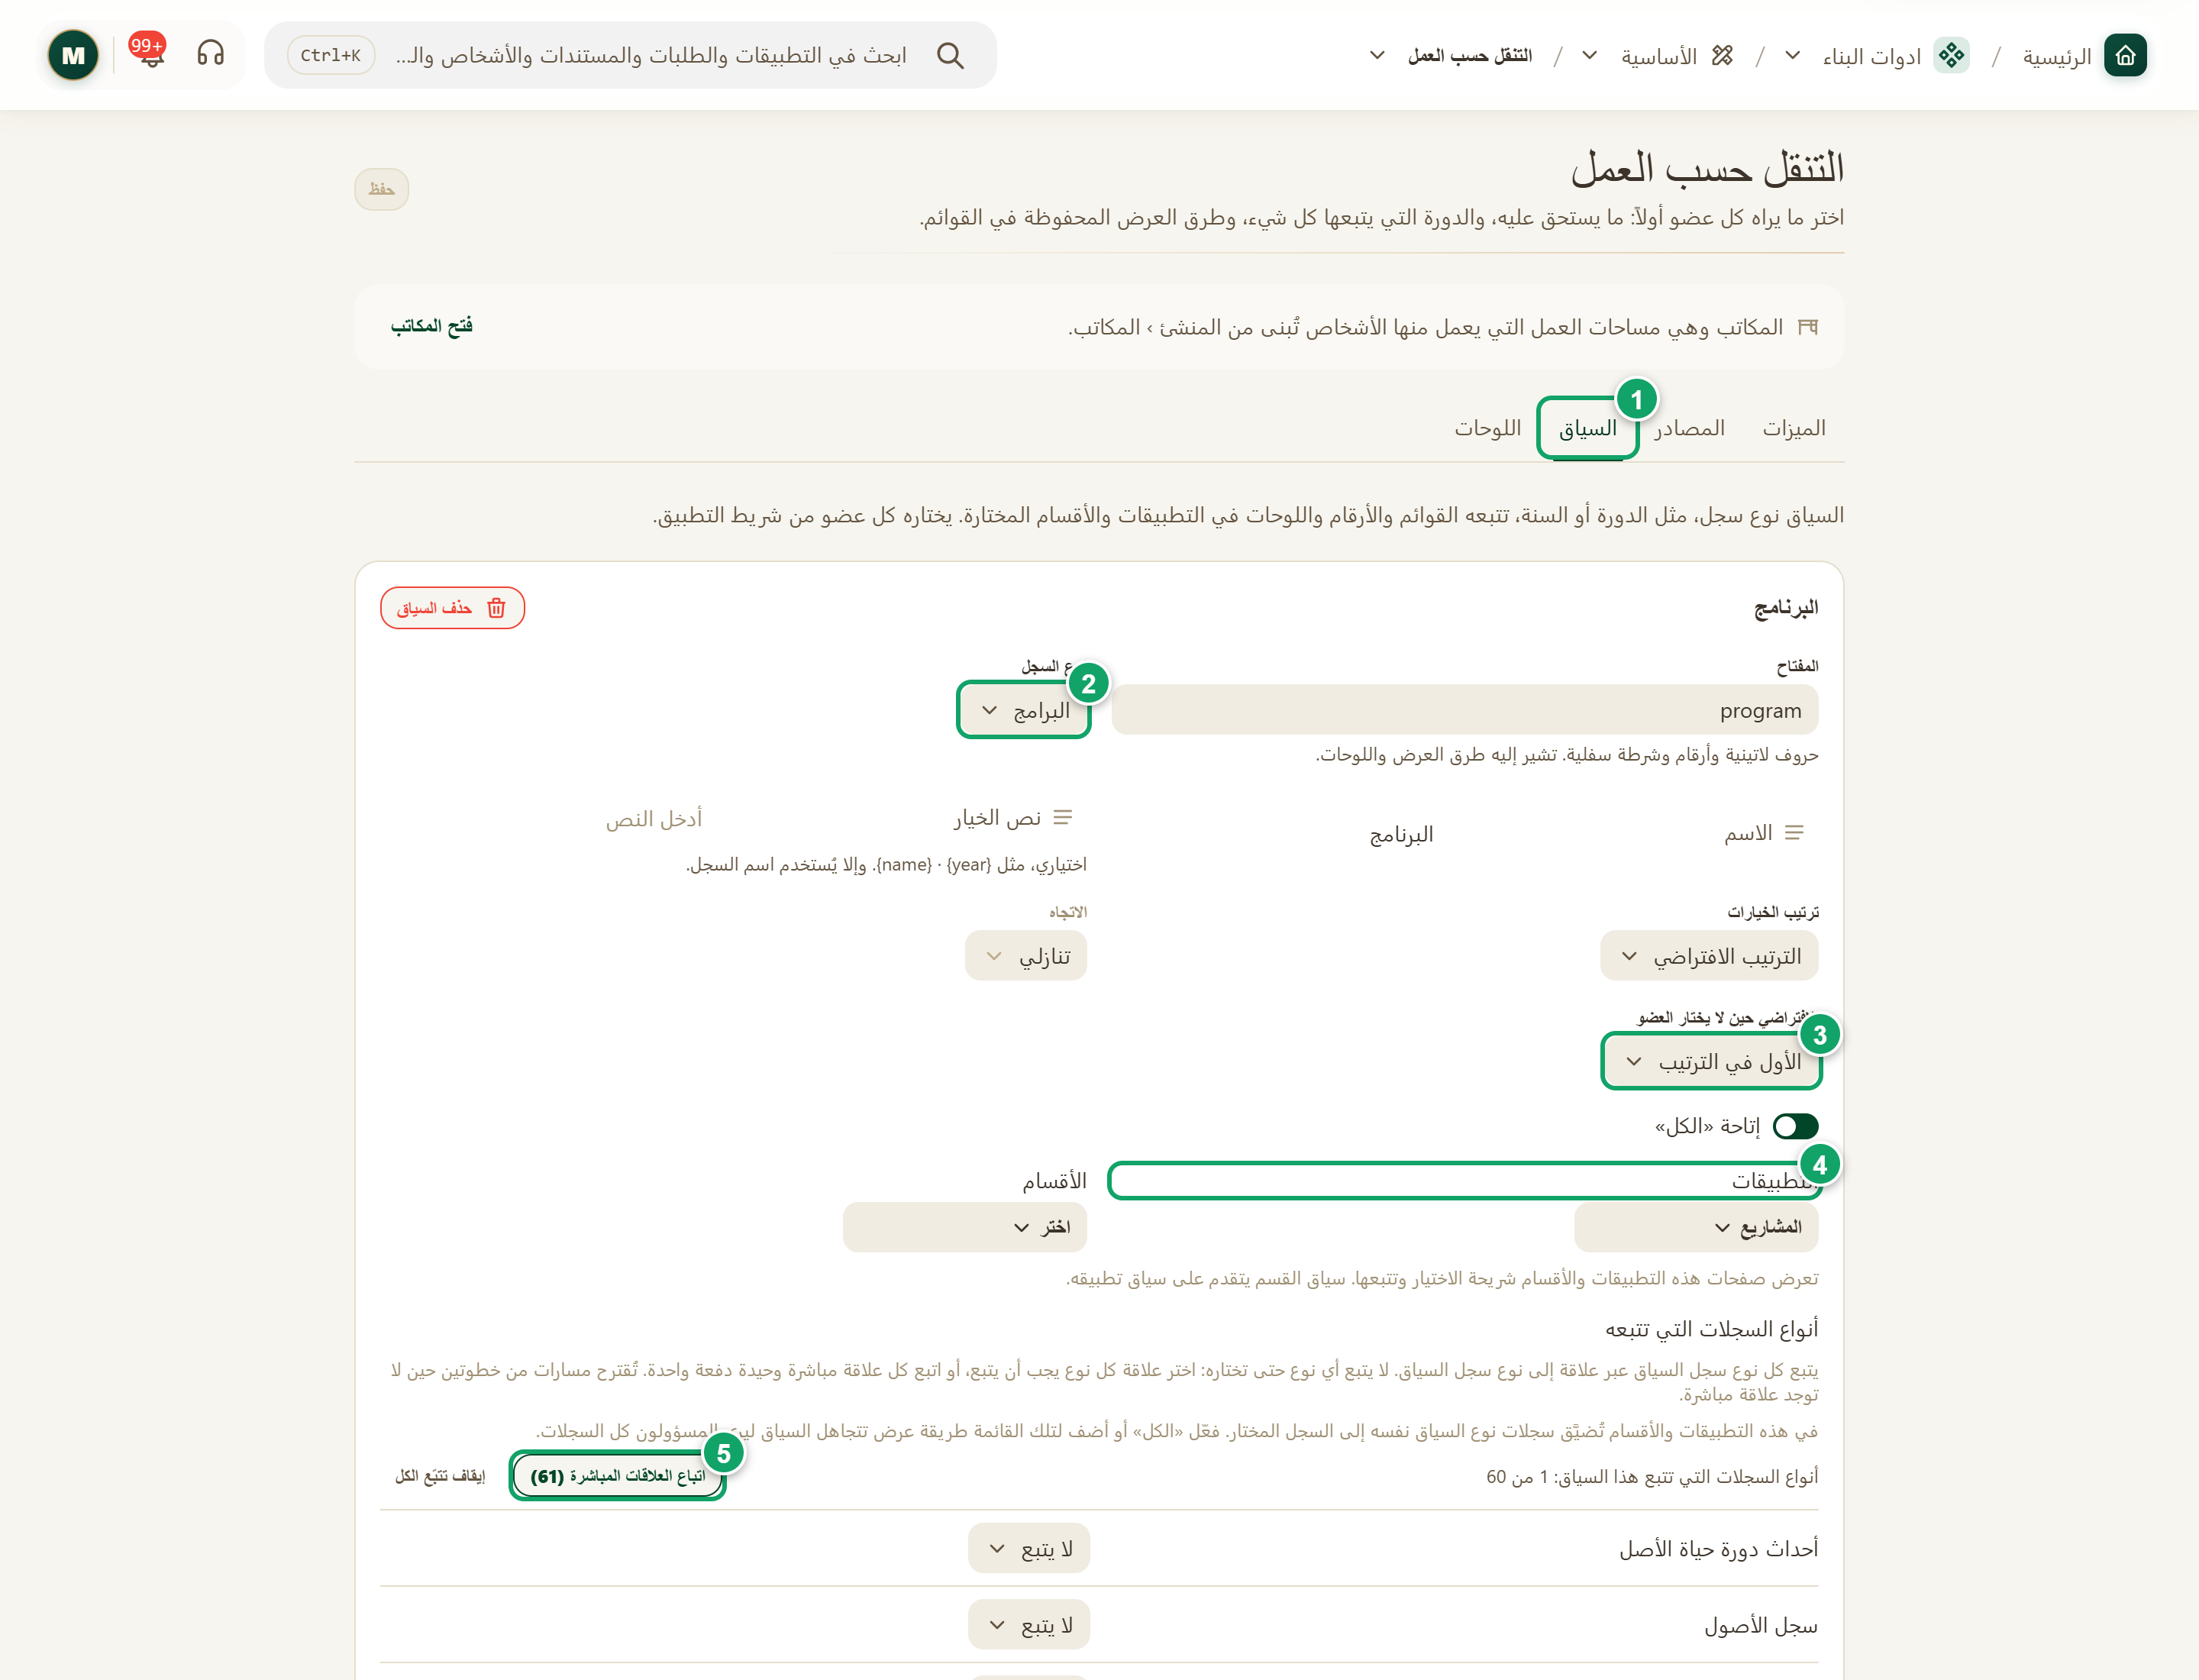
\includegraphics[width=0.95\linewidth,height=0.72\textheight,keepaspectratio]{figures/screens/ch06-wn-context-ar.png}
\caption{تبويب «السياق»}
\label{fig:builder-work-navigation-context-screen}
\shotnote{تعرض الصورة تبويب «السياق» في مؤسسة الاختبار، وفيه سياق باسم «البرنامج» مبني على نوع السجلات «البرامج» ويتبعه تطبيق «المشاريع». ويظهر في أسفله جدول «أنواع السجلات التي تتبعه»، وأغلب أنواعه على «لا يتبع» لأن التتبع لا يبدأ حتى تختاره. ① «السياق»: التبويب الذي تضبط فيه السياقات. ② «نوع السجل»: نوع الدورات أو السنوات الذي يُبنى عليه السياق. ③ «الافتراضي حين لا يختار العضو»: القيمة المعروضة قبل أن يختار العضو. ④ «التطبيقات»: الأماكن التي تعرض الشريحة وتتبعها، وبجانبها «الأقسام». ⑤ «اتباع العلاقات المباشرة»: يختار كل علاقة مباشرة وحيدة دفعة واحدة.}
\end{figure}

\begin{table}[H]
\centering
\caption{إعدادات السياق}
\label{tab:builder-work-navigation-context-fields}
\begin{tabularx}{\linewidth}{R{3.6cm} Y}
\rcHeaderRow
\thh{الإعداد} & \thh{ما يحدده}\\
المفتاح ونوع السجل والاسم & «المفتاح» معرّف تشير إليه طرق العرض واللوحات، و«نوع السجل» هو نوع الدورات أو السنوات، و«الاسم» هو ما يراه العضو.\\
نص الخيار & صيغة اختيارية لنص كل خيار في الشريحة. وإذا تُرك فارغاً يُستخدم اسم السجل.\\
ترتيب الخيارات والاتجاه & الحقل الذي تُرتَّب به الخيارات، و«تصاعدي» أو «تنازلي».\\
الافتراضي حين لا يختار العضو & «الأول في الترتيب»، أو «الأول في حالة معينة» مع «حقل الحالة» و«الحالات»، أو «لا شيء (عرض الكل)».\\
إتاحة «الكل» & يضيف إلى الشريحة خياراً يعرض كل السجلات دون تضييق.\\
التطبيقات والأقسام & الأماكن التي تعرض الشريحة وتتبعها. وسياق القسم يتقدم على سياق تطبيقه.\\
أنواع السجلات التي تتبعه & لكل نوع سجلات تختار في «يتبع عبر» العلاقة التي يتبع بها السياق، أو تختار «لا يتبع». ويختار زر «اتباع العلاقات المباشرة» كل علاقة مباشرة وحيدة دفعة واحدة.\\
\end{tabularx}
\end{table}

\begin{rcwarn}[لا يتبع أي نوع حتى تختاره]
إضافة التطبيق إلى السياق لا تكفي وحدها؛ فلا يتضيق نوع سجلات حتى تختار له علاقة في «أنواع السجلات التي تتبعه». ثم إن سجلات نوع السياق نفسه تتضيق إلى القيمة المختارة في تلك الأماكن، لذلك فعّل «الكل» حتى يستطيع المسؤولون رؤية كل السجلات.
\end{rcwarn}

\begin{figure}[H]
\centering
\begin{tikzpicture}[node distance=0.5cm]
\node[stepBox] (a) {\RL{تشغيل مبدّل السياق}};
\node[stepBox,below=of a] (b) {\RL{إضافة سياق}};
\node[stepBox,below=of b] (c) {\RL{نوع السجل والافتراضي}};
\node[stepBox,below=of c] (d) {\RL{التطبيقات والأقسام}};
\node[stepBox,below=of d] (e) {\RL{الأنواع التي تتبعه}};
\node[stepBox,below=of e] (f) {\RL{حفظ}};
\draw[flowsTo] (a) -- (b);
\draw[flowsTo] (b) -- (c);
\draw[flowsTo] (c) -- (d);
\draw[flowsTo] (d) -- (e);
\draw[flowsTo] (e) -- (f);
\end{tikzpicture}
\rclegend
\caption{ضبط سياق مشترك}
\label{fig:builder-work-navigation-context-flow}
\shotnote{يبدأ المخطط بتشغيل الميزة لأن الشريحة لا تظهر للأعضاء من دونها، حتى لو كان السياق مضبوطاً. ويضع اختيار الأنواع التابعة بعد الأماكن، لأن المكان يحدد أين تظهر الشريحة، أما العلاقة فتحدد أي السجلات تتضيق فعلاً.}
\end{figure}

\subsection{خطوات العمل والتحقق}
\begin{enumerate}
\item شغّل «مبدّل السياق» في تبويب «الميزات».
\item افتح تبويب «السياق» واضغط «إضافة سياق»، ثم اكتب «المفتاح» واختر «نوع السجل» واكتب «الاسم».
\item اختر «الافتراضي حين لا يختار العضو»، وفعّل «إتاحة «الكل»» عند الحاجة.
\item اختر «التطبيقات» و«الأقسام» التي تتبعه، ثم اختر لكل نوع سجلات العلاقة التي يتبع عبرها.
\item اضغط «حفظ» في رأس الصفحة.
\end{enumerate}

\textbf{تحقق ومعالجة المشكلة:} بعد الحفظ وإعادة تحميل الصفحة، تظهر الشريحة في شريط التطبيقات المختارة، وتتضيق قوائمها عند اختيار قيمة. فإذا لم تتضيق قائمة ما، فارجع إلى «أنواع السجلات التي تتبعه» وتأكد من أن نوعها لا يحمل «لا يتبع». وإذا ظهر بجانب تطبيق «يتبع «…» مسبقاً»، فهو تابع لسياق آخر، فأزله من ذلك السياق أولاً.

\clearpage
\section{نطاق بيانات اللوحات}
\label{sec:builder-feature-work-navigation-dashboards}

تعرض لوحة المعلومات أرقاماً ورسوماً محسوبة من السجلات. ويحدد «نطاق البيانات» السجلات التي تُحسب منها: إما «بصلاحيات المشاهد»، فيرى كل شخص أرقاماً من السجلات التي يحق له رؤيتها فقط، وإما «بيانات المنظمة كاملة»، فيرى كل من يفتح اللوحة أرقام كل السجلات.

ويضبط هذا التبويب أمرين: النطاق الذي تُنشأ به اللوحات الجديدة، وقائمة اللوحات الحالية التي ما زالت تعرض بيانات المؤسسة كاملة، مع إمكانية تحويلها إلى صلاحيات المشاهد.

\textbf{المسار ومن يستخدمه:} «ادوات البناء» ← «الأساسية» ← «التنقل حسب العمل» ← «اللوحات». ولا يرى قائمة اللوحات إلا مالكو المؤسسة ومسؤولوها.

\begin{rcnote}[مثال: شركة الأفق]
يجد مسؤول النظام في القائمة لوحة الزيارات التي تعرض أرقام الفرعين لكل من يفتحها. فيحوّلها إلى صلاحيات المشاهد، فيرى عمر حداد أرقام طلباته فقط، بينما ترى سارة الخطيب ما تسمح به صلاحياتها. ويحوّل اللوحة من ④.
\end{rcnote}

\begin{figure}[H]
\centering
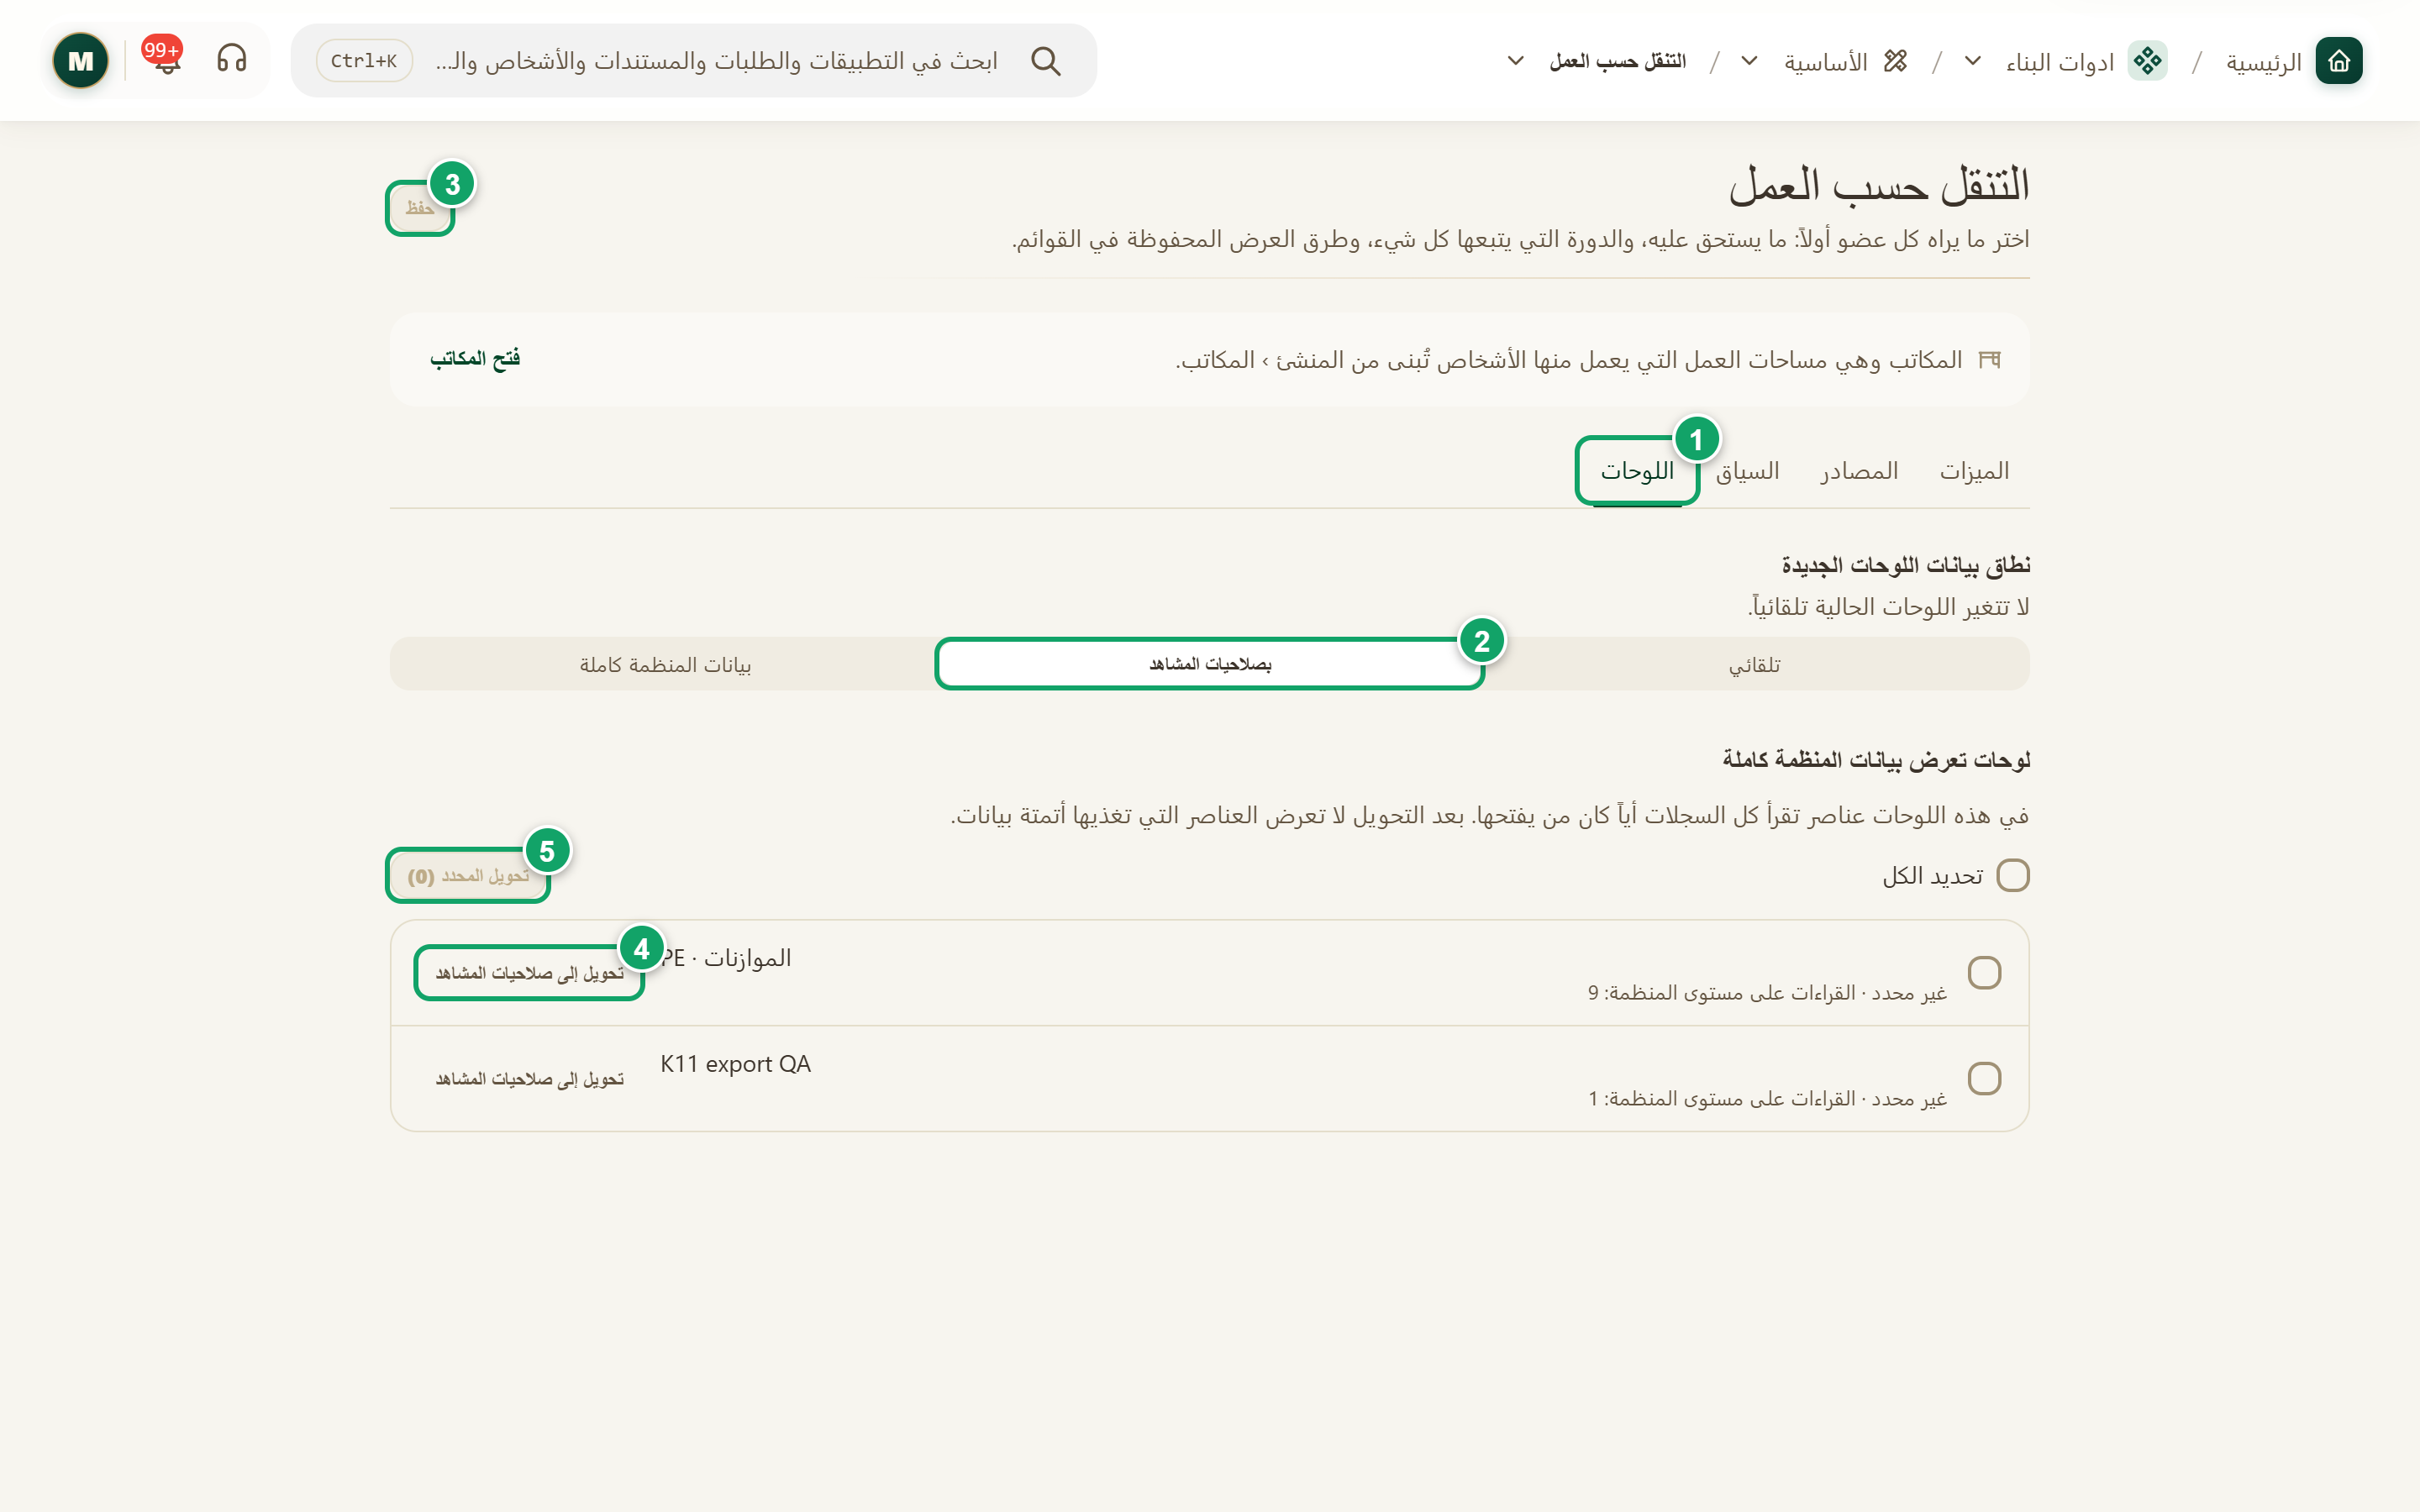
\includegraphics[width=0.95\linewidth,height=0.72\textheight,keepaspectratio]{figures/screens/ch06-wn-dashboards-ar.png}
\caption{تبويب «اللوحات»}
\label{fig:builder-work-navigation-dashboards-screen}
\shotnote{تعرض الصورة تبويب «اللوحات» في مؤسسة الاختبار، ونطاق اللوحات الجديدة فيه «بصلاحيات المشاهد»، بينما تبقى في القائمة لوحتان تقرآن بيانات المؤسسة كاملة مع عدد هذه القراءات. ويبيّن ذلك أن اختيار النطاق لا يغيّر اللوحات الحالية، وأن تحويلها خطوة مستقلة تُنفَّذ فوراً. ① «اللوحات»: التبويب. ② «بصلاحيات المشاهد»: نطاق اللوحات الجديدة. ③ «حفظ»: يحفظ اختيار النطاق. ④ «تحويل إلى صلاحيات المشاهد»: يحوّل لوحة واحدة. ⑤ «تحويل المحدد»: يحوّل كل اللوحات التي حددتها.}
\end{figure}

\begin{table}[H]
\centering
\caption{محتوى تبويب «اللوحات»}
\label{tab:builder-work-navigation-dashboards-parts}
\begin{tabularx}{\linewidth}{R{3.6cm} Y}
\rcHeaderRow
\thh{الجزء} & \thh{ما يفعله}\\
نطاق بيانات اللوحات الجديدة & «تلقائي» أو «بصلاحيات المشاهد» أو «بيانات المنظمة كاملة». والتلقائي يعني صلاحيات المشاهد ما دامت إحدى ميزات التنقل حسب العمل مفعّلة. ولا تتغير اللوحات الحالية بهذا الاختيار.\\
لوحات تعرض بيانات المنظمة كاملة & قائمة باللوحات التي فيها عناصر تقرأ كل السجلات أياً كان من يفتحها، مع عدد هذه القراءات لكل لوحة.\\
تحويل إلى صلاحيات المشاهد & يحوّل لوحة واحدة، أو يحوّل «تحويل المحدد» كل اللوحات التي حددتها. ويُنفَّذ التحويل فوراً دون انتظار «حفظ».\\
\end{tabularx}
\end{table}

\begin{rcwarn}[قبل التحويل]
بعد التحويل لا تعرض العناصر التي تغذيها أتمتة أي بيانات، لأن الأتمتة لا تعمل بصلاحيات المشاهد. لذلك راجع اللوحة بعد تحويلها، وأعد بناء هذه العناصر إن احتجت إليها.
\end{rcwarn}

\begin{figure}[H]
\centering
\begin{tikzpicture}[node distance=0.5cm]
\node[stepBox] (a) {\RL{اختيار نطاق اللوحات الجديدة}};
\node[stepBox,below=of a] (b) {\RL{حفظ}};
\node[stepBox,below=of b] (c) {\RL{مراجعة قائمة اللوحات}};
\node[stepBox,below=of c] (d) {\RL{تحويل إلى صلاحيات المشاهد}};
\node[stepBox,below=of d] (e) {\RL{فتح اللوحة ومراجعتها}};
\draw[flowsTo] (a) -- (b);
\draw[flowsTo] (b) -- (c);
\draw[flowsTo] (c) -- (d);
\draw[flowsTo] (d) -- (e);
\end{tikzpicture}
\rclegend
\caption{ضبط نطاق بيانات اللوحات}
\label{fig:builder-work-navigation-dashboards-flow}
\shotnote{يفصل المخطط بين إجراءين يُحفظان بطريقتين مختلفتين: فنطاق اللوحات الجديدة يُحفظ مع بقية الصفحة بزر «حفظ»، أما التحويل فيُطبَّق على اللوحة فوراً. لذلك تنتهي السلسلة بفتح اللوحة للتأكد من أن عناصرها ما زالت تعرض ما يُنتظر منها.}
\end{figure}

\subsection{خطوات العمل والتحقق}
\begin{enumerate}
\item افتح «التنقل حسب العمل»، ثم تبويب «اللوحات».
\item اختر في «نطاق بيانات اللوحات الجديدة» القيمة المناسبة، ثم اضغط «حفظ» في رأس الصفحة.
\item راجع «لوحات تعرض بيانات المنظمة كاملة»، وحدد اللوحات التي يجب أن تعرض لكل شخص ما يخصه.
\item اضغط «تحويل إلى صلاحيات المشاهد» في صف اللوحة، أو «تحويل المحدد».
\end{enumerate}

\textbf{تحقق ومعالجة المشكلة:} بعد التحويل تظهر رسالة «حُوّلت إلى صلاحيات المشاهد:» مع العدد، وتختفي اللوحة من القائمة. وعندما تخلو القائمة تظهر «لا توجد لوحة تعرض بيانات المنظمة كاملة.». فإذا ظهرت «تعذر تحويل اللوحات.»، فأعد المحاولة؛ وإذا لم تظهر القائمة أصلاً، فاطلب من مالك المؤسسة أو مسؤولها فتح التبويب.

\clearpage
\section{إعدادات تحتاج إلى مراجعة}
\label{sec:builder-feature-work-navigation-stale}

تشير إعدادات «التنقل حسب العمل» إلى أشياء موجودة في أماكن أخرى: أنواع سجلات وحقول وانتقالات وأدوار وتطبيقات وأقسام. فإذا حُذف أحدها أو تغيّر نوعه، يصبح الإعداد الذي يشير إليه غير صالح. لذلك تفحص الصفحة إعداداتها عند فتحها، وتعرض ما يحتاج إلى إصلاح قبل أن يلاحظ الأعضاء خللاً في قوائمهم.

ويرفض الحفظ أي إعداد يشير إلى شيء غير موجود، فلا يُحفظ شيء حتى تصلحه.

\textbf{المسار ومن يستخدمه:} «ادوات البناء» ← «الأساسية» ← «التنقل حسب العمل»، ثم التبويب المعلَّم بالتنبيه. يستخدمه مالك المؤسسة ومسؤولها بعد تعديل أنواع السجلات أو الأدوار.

\begin{rcnote}[مثال: شركة الأفق]
يحذف مسؤول النظام حقل «المراجِع» من «طلبات الزيارة»، فتظهر في «التنقل حسب العمل» رسالة «إعدادات تحتاج إلى مراجعة: 1». فيفتح «المصادر» ويجد في المصدر «الحقل غير موجود» مع السبب «الحقل لم يعد موجوداً»، فيختار حقلاً آخر ويحفظ.
\end{rcnote}

\begin{table}[H]
\centering
\caption{الرسائل التي قد تظهر}
\label{tab:builder-work-navigation-stale-messages}
\begin{tabularx}{\linewidth}{R{3.6cm} Y}
\rcHeaderRow
\thh{الرسالة} & \thh{معناها وما تفعله}\\
إعدادات تحتاج إلى مراجعة & عدد الإعدادات التي تشير إلى شيء حُذف أو تغيّر. ويُعلَّم كل تبويب فيه مشكلة، ويظهر تحت الإعداد سطر يذكر العنصر وسبب المشكلة.\\
تعذرت قراءة الإعدادات المخزنة & الإعدادات المحفوظة تالفة، فتعمل كل الميزات كأنها متوقفة. والحفظ هنا يستبدلها بما تضبطه في الصفحة.\\
حفظ شخص آخر هذه الإعدادات بعد أن فتحتها & لم يُحفظ شيء. اضغط «إعادة التحميل» لترى تغييراته، وستضيع تعديلاتك غير المحفوظة.\\
\end{tabularx}
\end{table}

\begin{table}[H]
\centering
\caption{أسباب شائعة}
\label{tab:builder-work-navigation-stale-reasons}
\begin{tabularx}{\linewidth}{R{3.6cm} Y}
\rcHeaderRow
\thh{السبب} & \thh{الإصلاح}\\
نوع السجل لم يعد موجوداً & اختر نوع سجلات آخر للمصدر أو السياق، أو احذف الإعداد.\\
الحقل لم يعد موجوداً & اختر الحقل الذي حل محله في نافذة المصدر.\\
لم يعد حقل حالة أو تاريخ أو علاقة أو عضو & تغيّر نوع الحقل في المنشئ، فاختر حقلاً من النوع المطلوب.\\
حُذف الدور أو التطبيق أو القسم & أزل العنصر المحذوف من «الأدوار التي تراه» أو من أماكن السياق.\\
\end{tabularx}
\end{table}

\begin{figure}[H]
\centering
\begin{tikzpicture}[node distance=0.5cm]
\node[stepBox] (a) {\RL{قراءة عدد الإعدادات}};
\node[stepBox,below=of a] (b) {\RL{فتح التبويب المعلَّم}};
\node[stepBox,below=of b] (c) {\RL{قراءة العنصر والسبب}};
\node[stepBox,below=of c] (d) {\RL{تعديل الإعداد أو حذفه}};
\node[stepBox,below=of d] (e) {\RL{حفظ}};
\draw[flowsTo] (a) -- (b);
\draw[flowsTo] (b) -- (c);
\draw[flowsTo] (c) -- (d);
\draw[flowsTo] (d) -- (e);
\end{tikzpicture}
\rclegend
\caption{إصلاح إعداد يشير إلى عنصر محذوف}
\label{fig:builder-work-navigation-stale-flow}
\shotnote{يوضّح المخطط أن الإصلاح يبدأ من التبويب المعلَّم، لأن كل مشكلة تظهر بجانب الإعداد الذي سببها. وينتهي بالحفظ لأن الصفحة لا تقبل حفظ أي تعديل آخر ما دامت مشكلة واحدة باقية.}
\end{figure}

\subsection{خطوات العمل والتحقق}
\begin{enumerate}
\item افتح «التنقل حسب العمل»، واقرأ عدد «إعدادات تحتاج إلى مراجعة».
\item افتح التبويب الذي يحمل علامة التنبيه، وابحث عن السطر الأحمر تحت الإعداد.
\item اقرأ العنصر وسبب المشكلة، ثم اضغط «تعديل» في صف المصدر أو عدّل السياق مباشرة.
\item اختر عنصراً موجوداً بدلاً من المحذوف، أو احذف الإعداد إذا لم يعد مطلوباً، ثم اضغط «حفظ».
\end{enumerate}

\textbf{تحقق ومعالجة المشكلة:} بعد الحفظ تختفي رسالة «إعدادات تحتاج إلى مراجعة» وعلامات التبويبات، وتظهر «تم حفظ التنقل حسب العمل». فإذا ظهرت «تعذر حفظ الإعدادات.» مع «بعض الإعدادات غير صالحة:»، فاقرأ القائمة التي تليها وأصلح كل بند فيها. وإذا ظهرت رسالة التعارض، فاضغط «إعادة التحميل» ثم أعد تعديلك.
